\chapter{The GOTO Telescope Control System}
\label{chap:gtecs}
\chaptoc{}

% ########################################

\newpage
\section{Introduction}
\label{sec:gtecs_intro}
\begin{colsection}

% ~~~~~~~~~~~~~~~~~~~~

\begin{colsection}

In this chapter I outline my work creating a control system for the GOTO telescope. \aref{sec:gtecs}, \aref{sec:hardware_control} and \aref{sec:autonomous} are expanded from my SPIE conference paper \citealt{Dyer}. The GOTO Telescope Control System is based on the pt5m control system (\citealt{pt5m}), written primarily by Tim Butterly at Durham and Stu Littlefair and Vik Dhillon at Sheffield. This provided the foundation that the GOTO system builds upon, but has been heavily modified and rewritten to meet the requirements of the GOTO project. All work described in this chapter is my own, incorporating advice and feedback from members of the GOTO collaboration.

\end{colsection}

% ~~~~~~~~~~~~~~~~~~~~

\subsection{Requirements of the control system}
\label{sec:control_requirements}
\begin{colsection}

My first task as part of the GOTO collaboration, in the summer of 2015 before I started my PhD in Sheffield, was to decide on what control system software to use for the telescope. There were several requirements to consider.

First, the chosen system had to allow for remote and, most importantly, robotic operation of GOTO.\@ There are many telescope control software packages available, but the majority are designed for a human observer to operate. GOTO however was to be a fully autonomous telescope, which meant operating nightly with no human intervention. This meant the control system had to contain routines for observing targets and standard tasks like taking calibration frames. On top of that it was desirable for the system to be able to monitor itself to detect and fix any errors as much as possible without the need for human intervention. Finally it had to be able to monitor and react to external conditions, for example closing the dome if rain was detected.

Second, the system had to include an observation scheduler, which could decide what the telescope should observe during the night. A basic scheduler might be run in the evening to create a night plan, as observers typically do when operating a telescope. However that function alone would not meet the expected operations required from GOTO:\@ normally carrying out an all-sky survey but with a robust interrupt protocol for gravitational wave follow-up. The system therefore had to be able to recalculate what to observe on-the-fly, and be able to react immediately to transient \gls{too} events.

Furthermore, although the project was still at an early stage the idea of linking together multiple telescopes into a global network was also considered, and the chosen control system would ideally be expandable to facilitate this in the future.

There were also several physical considerations when it came to choosing between software systems. The telescope hardware had already been decided on: an Astrohaven clamshell dome\footnote{Astro Haven Enterprises, CA, USA;\@ (\url{www.astrohaven.com})}, a custom mount with a \gls{sitech} servo controller\footnote{Sidereal Technology, OR, USA;\@ (\url{www.siderealtechnology.com})} and multiple unit telescopes all equipped with \gls{fli} cameras, focusers and filter wheels\footnote{Fingerlake Instruments, NY, USA;\@ (\url{www.flicamera.com})}. Any control system would need to communicate with all of this hardware, so any software package with existing drivers would be desirable. \rtxt{in intro}

Two particular hardware-related challenges faced the control system project. The first was that the SiTech controller software, \software{SiTechEXE}, only ran on Microsoft Windows. The software did have an accessible \gls{api} through the \software{ASCOM} standard\footnote{\url{www.ascom-standards.org}}, but that still required some form of the mount control system to be running on Windows. As most professional scientific software in astronomy runs on Linux systems, this lead to two options: either have just a small interface running on the Windows machine and the rest of the system on Linux, or have the entire system run on Windows.

The second hardware-related challenge was to deal with the multiple-unit telescope design of \gls{goto}. A full array of eight unit telescopes (UTs) would require eight cameras, focusers and filter wheels. These would all need to be run in parallel, most importantly there needed to be no delay between the exposures starting and finishing on each camera. The physical construction of the telescope also came into play. The \gls{fli} units all require a USB connection to the control computer. A single computer situated in the dome would therefore require 24 extra-long USB cables to run up the mount. The suggested solution was to have small computers attached to the mount boom arms to act as intermediate interfaces to the \gls{ut} hardware \rtxt{shown in figure in intro}. The control system therefore needed to be able to run in a distributed manner across multiple computers, potentially even running different operating systems.

There were also practical details to consider when choosing the control software. \gls{goto} was designed as a relatively inexpensive project that could be built quickly and copied across multiple sites, therefore any costly software licenses should ideally be avoided. Experience and support requirements should also be considered, and reusing a software system that members of the collaboration had experience with would provide benefits compared to a completely new system.

\end{colsection}

% ~~~~~~~~~~~~~~~~~~~~

\subsection{Different control system options}
\label{sec:control_options}
\begin{colsection}

Four possible options for the GOTO control system were considered: the existing software packages \software{ACP Expert}, \software{Talon} and \software{RTS2}, or a custom system based on the code written for the \gls{pt5m}. At the July 2015 GOTO meeting at Warwick University I gave a talk outlining the control system requirements and presenting the four options, and the decision taken was to adapt the \gls{pt5m} system for use by GOTO.\@ The three rejected systems are described below, while the \gls{pt5m} system is described in more detail in \aref{sec:pt5m}.

\subsubsection{\software{ACP Expert}}
\software{ACP Expert}\footnote{\url{http://acp.dc3.com}} is a commercial observatory control software system by DC3-Dreams. It is used by some advanced amateur astronomers and a few scientific and university telescopes, such as the Open University's \gls{pirate} \citep{PIRATE}. As a complete Windows software package with a web interface it is marketed as being straightforward to use, in either remote or fully robotic modes. It uses the \software{ASCOM} standard library and DC3-Dreams also provide professional support and updates. This however came at a cost: \$2495 for the base software, plus an additional \$599 for Maxim DL camera control and \$650 per year for continued support. At the time, \gls{goto} was anticipated to be deployed in a matter of months, so the quick and simple pre-existing commercial solution was tempting. However it was unclear if the \software{ACP} software would be able to cope with \gls{goto}'s unusual design, and its closed-source model would restrict our ability to make modifications.

\subsubsection{\software{Talon}}

The \software{Talon} observatory control system\footnote{\url{https://observatory.sourceforge.io}} is a Linux-based, open-source system created by \gls{omi}. It was included as an option primarily as at the time it was the control system of choice for the other observatories operated by Warwick University, such as SuperWASP \citep{SuperWASP}. \gls{omi} had built the SuperWASP mount and developed \software{Talon} alongside it, before later making it open source. However development of \software{Talon} has been almost non-existent over the past decade, and when building the \gls{ngts} a large amount of custom software was needed to allow \software{Talon} to work with its multiple telescopes \citep{ngts}. Warwick were already looking at replacing \software{Talon} for their \gls{w1m} and when upgrading SuperWASP.\@ Therefore adopting it for \gls{goto} would be unlikely and even counter-productive, as whatever was chosen for \gls{goto} was expected to (and ultimately did) influence and benefit the concurrent development of a new control system for \gls{w1m}.

\subsubsection{\software{RTS2}}

The \gls{rts2}\footnote{\url{https://rts2.org}} \citep{RTS2, RTS2b} is another free and open-source Linux software package. Unlike \software{Talon}, \software{RTS2} is under active development and is used by telescopes and observatories around the world \citep{BORAT, BOOTES-3, antarctic, ARTN}. There is a small but active user community and drivers for the hardware \gls{goto} would use had already been developed. The first version of RTS was written in \proglang{Python}, while the second version was rewritten in \proglang{C++} but with a \proglang{Python} interface available. \gls{rts2} was an attractive choice, however like the others it was unclear if it could be easily modified to meet the requirements for \gls{goto}'s multiple telescopes and Windows-controlled mount and no one in the collaboration had prior experience of using or implementing it.

\end{colsection}

% ~~~~~~~~~~~~~~~~~~~~

\subsection{The \textit{pt5m} control system}
\label{sec:pt5m}
\begin{colsection}

Built and operated by Sheffield and Durham Universities, \gls{pt5m} is a \SI{0.5}{\metre} telescope located on the roof of the \SI{4.2}{\metre} \gls{wht} on La Palma \citep{pt5m}. The telescope was originally developed as a \gls{slodar} system for atmospheric turbulence profiling in support of the CANARY laser guide star project on the \gls{wht} \citep{SLODAR_LaPalma, CANARY}. There are several \gls{slodar} telescopes around the world operated by Durham, including one in Korea that had just been commissioned at the time I joined the GOTO project \citep{SLODAR_Korea}. In order to make the most of the telescope when not being used for \gls{slodar} observations a science camera was added to \gls{pt5m} by Sheffield, and in-house control software was written to enable robotic observations. It has successfully been used for automatic observations of transient events since 2012, as well as being used for undergraduate teaching at Sheffield and Durham. All of the \gls{slodar} telescopes used a custom control system developed at Durham, and a similar system was used by the teaching telescopes of the Durham Department of Physics that I worked with during my undergraduate program. The \gls{pt5m} control system had been modified by the team at Durham and Sheffield for robotic operation, which matched well with what we needed for \gls{goto}. For this reason, on top of the existing experience of the software, it was chosen to be the base for the GOTO control system.

The \gls{pt5m} control system is written in \proglang{Python} and was built around multiple independent background programs called \emph{daemons}. Each daemon controls one category of hardware, for example the dome, mount or CCD controller. A script called the \emph{pilot} sends commands to the daemons when the system is operating in robotic mode, and the decision of what to observe is taken by the \emph{scheduler} which picks targets out of a database and returns the highest priority to the pilot. Finally a separate script called the \emph{conditions monitor} checks the local weather conditions and tells the pilot to close the dome in bad weather. An overview of the pt5m control system architecture is shown in \aref{fig:pt5m_software}.

The basic framework of the pt5m control system was adopted for \gls{goto}, but with several changes. The major difference between \gls{pt5m} and \gls{goto} are the multiple unit telescopes, but the same software control system could be adapted through the creation of interface daemons which allow communication to the unit telescopes over the internal dome network. In fact the independent, distributed nature of the daemon system made it very easy to expand to have daemons running on physically separate machines but still communicating over the same local network, including on both Linux and Windows computers.

\begin{figure}[p]
\begin{center}
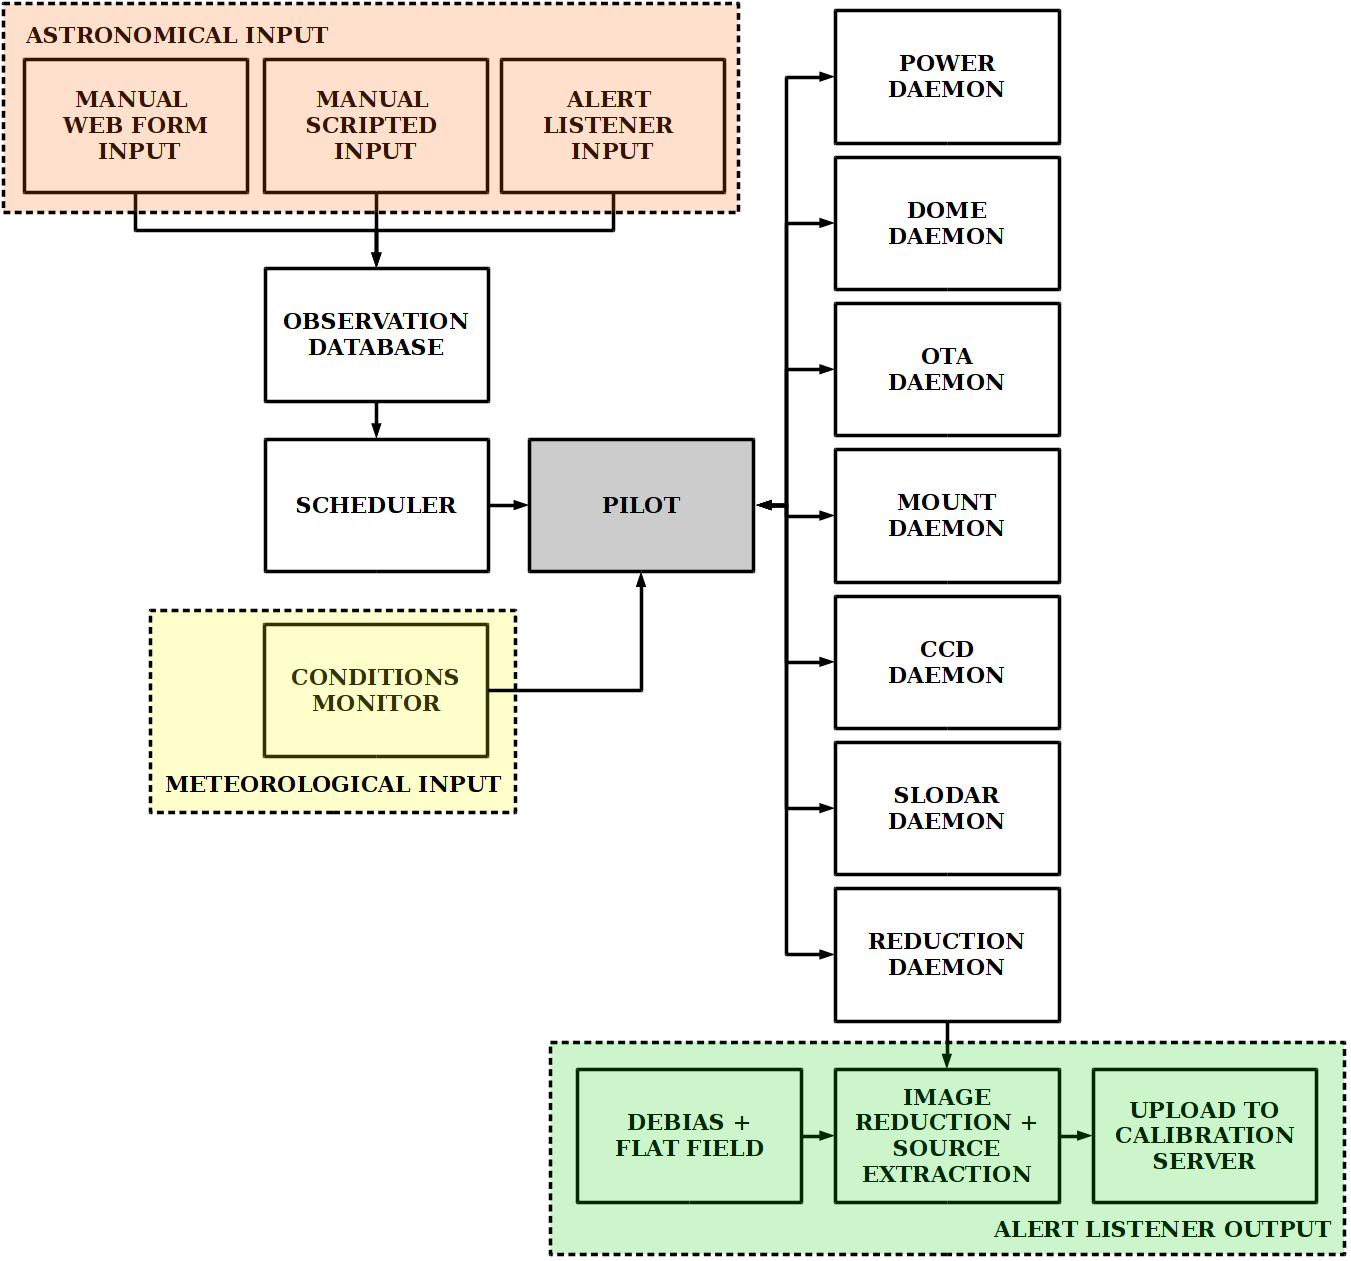
\includegraphics[width=\linewidth]{images/pt5m_software.png}
\end{center}
\caption[The pt5m control system architecture]{The \gls{pt5m} control system architecture, taken from \citet{pt5m}. The hardware daemons are shown on the right; they communicate with the pilot which receives information from the observation scheduler and the conditions monitor. This basic framework was adapted for the GOTO control system, c.f. \aref{fig:flow}.}
\label{fig:pt5m_software}
\end{figure}

\end{colsection}

% ~~~~~~~~~~~~~~~~~~~~

\end{colsection}

% ########################################

\newpage
\section{Overview of G-TeCS}
\label{sec:gtecs}
\begin{colsection}

% ~~~~~~~~~~~~~~~~~~~~

\begin{colsection}

The \gls{gtecs} is the name given to the collection of programs that have been developed to fulfil the requirements of the GOTO project given in \aref{sec:control_requirements}. The \gls{pt5m} control system as described in the previous section formed the basis for \gls{gtecs}. Its structure of multiple independent daemons was developed into the core system architecture of G-TeCS, shown in \aref{fig:flow}. This section gives an overview of the system and its implementation, and the following sections discuss in detail the two core branches of G-TeCS:\@ the base hardware control programs (\aref{sec:hardware_control}) and the autonomous systems built on top of them (\aref{sec:autonomous}).

\begin{figure}[p]
    \begin{center}
        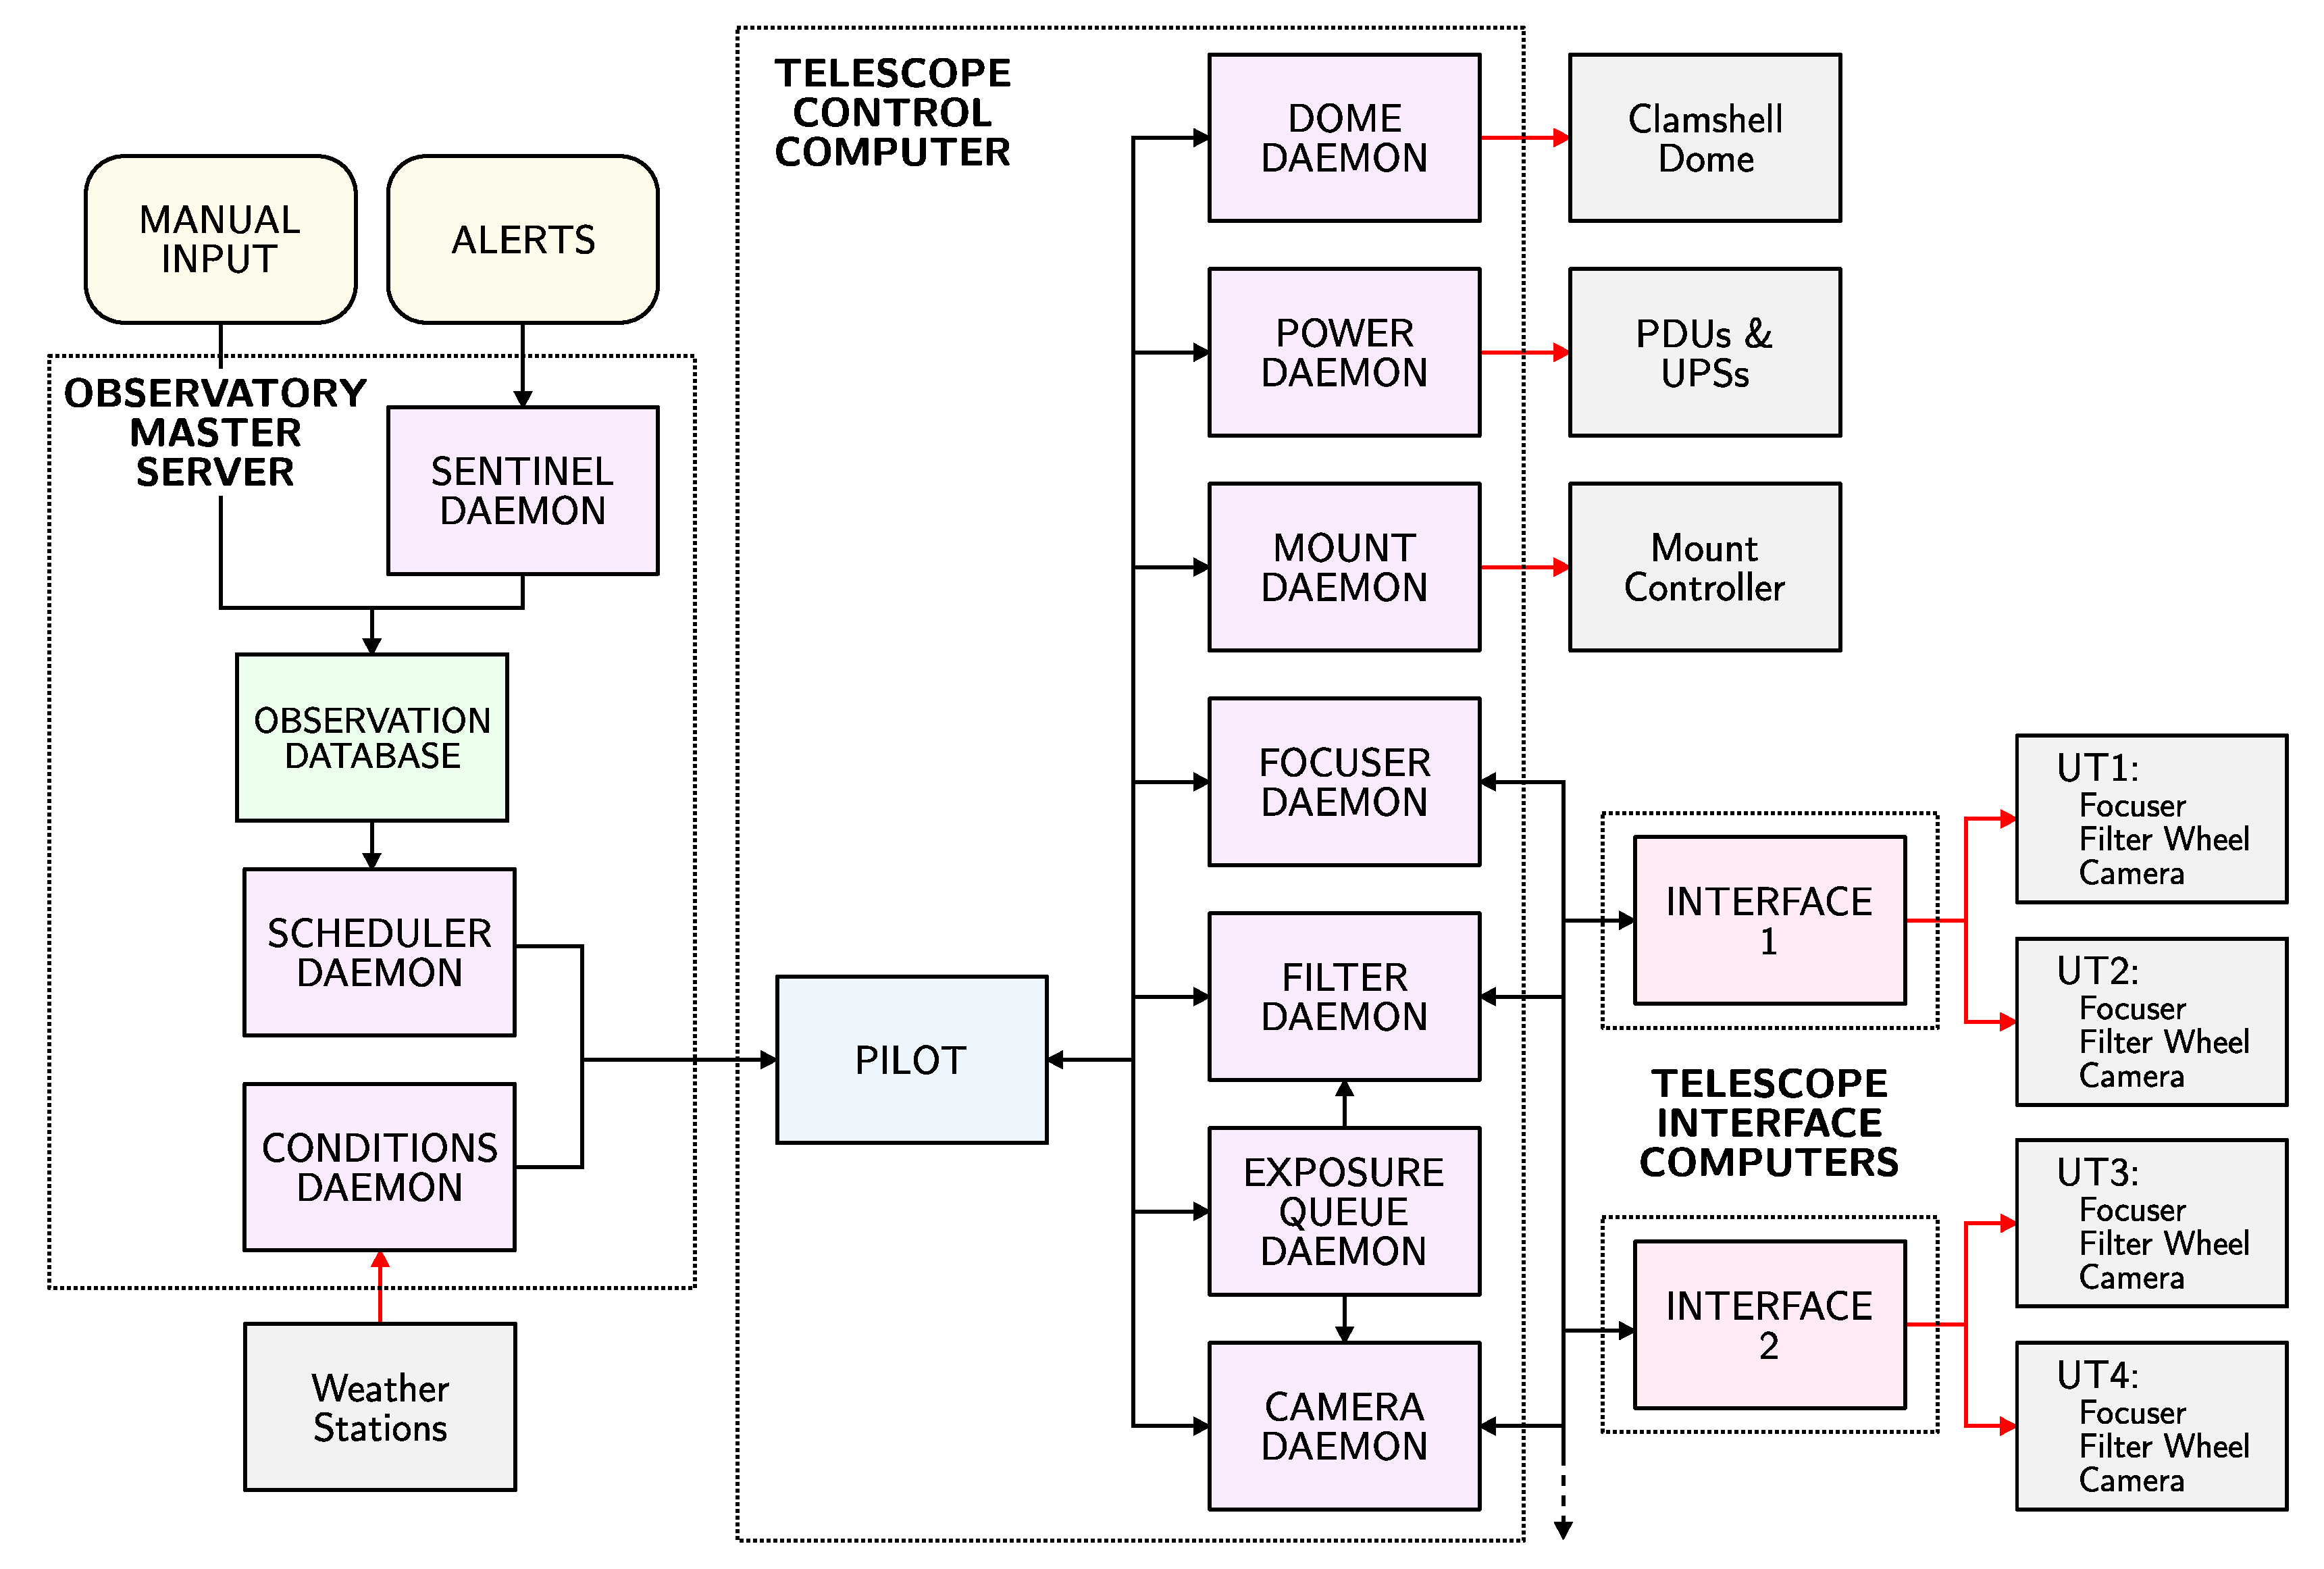
\includegraphics[width=\linewidth]{images/flow.pdf}
    \end{center}
    \caption[The G-TeCS system architecture]{
        The \gls{gtecs} system architecture as deployed on La Palma. The observation database as well as the sentinel, scheduler and conditions daemons shown to the left run on a central observatory-wide server located in the SuperWASP building next to the GOTO domes, while the pilot and hardware daemons are located on the telescope control computer within the dome. Control for the unit telescope hardware (focuser, filter wheel and camera) is sent via an interface daemon for each pair of UTs, running on computers attached to the mount. Only the system for the prototype instrument (one mount with four unit telescopes) is shown.
    }\label{fig:flow}
\end{figure}

\end{colsection}

% ~~~~~~~~~~~~~~~~~~~~

\subsection{Implementation}
\label{sec:implementation}
\begin{colsection}

The core \gls{gtecs} code is written as a \proglang{Python} package, \pkg{gtecs}. This includes all of the daemons, scripts, associated modules and functions. One core component, the code and functions to interact with the observation database (see \aref{sec:obsdb}), has been split off into a separate \proglang{Python} package ObsDB (\pkg{obsdb}); this was to allow other users to interact with the database without the need to install the entire \pkg{gtecs} package. In addition, the code for alert processing within the sentinel (see \aref{sec:sentinel}) is in a separate module, GOTO-alert (\pkg{gotoalert}). This is because it originated as a separate coding project developed by Alex Obradovic at Monash, that I then took over and integrated with the \gls{gtecs} sentinel. GOTO-alert is described in more detail in \aref{sec:gotoalert}.

G-TeCS and the associated packages are written almost entirely in \proglang{Python}, specifically \proglang{Python3}. \proglang{Python} is a versatile programming language that is increasingly common in astronomy, helped by the popular open-source Astropy Project \citep{astropy}. \proglang{Python} version 3.0 was released in 2008 and is infamously not backwards-compatible with \proglang{Python2}. The code for \gls{pt5m} was written in \proglang{Python2}, and therefore initially so was G-TeCS.\@ Over the subsequent years the G-TeCS code was re-written to be compatible with both \proglang{Python2} and \proglang{Python3}, which was possible due to the inbuilt \code{\_\_future\_\_} module in \proglang{Python2} and the \code{six} package. Eventually, the addition of new features added to \proglang{Python3}, such as the \pkg{asyncio} package (used heavily by the pilot) in version 3.5, and the imminent end-of-life of \proglang{Python2} in 2020 led to the dropping of \proglang{Python2} support. This is in line with most other scientific \proglang{Python} packages including \pkg{astropy}, which is no longer developed for \proglang{Python2}. % chktex 21

The \pkg{gtecs} and associated packages have multiple dependencies. Some of the most critical external packages (not included in the \proglang{Python} standard library) are \pkg{numpy} for mathematical and scientific structures, \pkg{astropy} for astronomical functions, \pkg{Pyro4} for communicating between daemons (see \aref{sec:daemons} below) \pkg{sqlalchemy} for \proglang{SQL} database management (see \aref{sec:obsdb}), \pkg{astroplan} for scheduling (see \aref{sec:scheduler}), \pkg{voeventparse} for handling VOEvents (see \aref{sec:voevents}) and \pkg{gototile}, a custom package written for GOTO for skymap processing (described in \aref{sec:gototile}).

\end{colsection}

% ~~~~~~~~~~~~~~~~~~~~

\subsection{Daemons}
\label{sec:daemons}
\begin{colsection}

The core elements of the control system are the daemons. A \emph{daemon} is a type of computer program that runs as a background process, continually cycling and awaiting any input from the user. This is in contrast to a \emph{script} which is run once (either by the system or a user), carries out a series of tasks in the foreground and then exits once it is completed. Common examples of daemons on a Unix-based system are \software{sshd}, which listens for and creates \gls{ssh} connections, and \software{cron}, which runs commands at predefined times. Incidentally both are used by G-TeCS:\@ \gls{ssh} commands are used to execute commands on remote machines and \software{cron} is used to run scripts like the pilot at a set time of day.

Daemons are the ideal form of software for hardware control. Once started each daemon runs continually as a background process, with a main control loop that repeats on a regular timescale (for the G-TeCS hardware daemons this is usually every \SI{0.1}{\second}). There are two primary tasks that are carried out within the loop by every daemon: monitoring the status of the hardware, and listening for and carrying out input commands. The former is typically not carried out every time the loop runs, because attempting to request and process the hardware status every \SI{0.1}{\second} would overwhelm the daemon and delay the loop. Instead the status checks are typically carried out every \SI{2}{\second}, or sooner if requested. By continually requesting the status of the hardware the daemon will detect very quickly if there are any problems, and should they be unable to reach their hardware they will enter an error state. However the daemons themselves will not attempt to self-diagnose and fix any problems that are detected, with the notable exception of the dome daemon (\aref{sec:dome}). Instead that is the job of the hardware monitors (see \aref{sec:pilot}); the daemons themselves will just report any problems to the pilot or user. The second reason for a control loop within the daemons is to listen for and carry out any commands issued to them. As these commands are dealt with within the loop it ensures only one command is carried out at a time; the alternative of user input going directly to the hardware could cause problems with overlapping commands. These commands can be as simple as querying the cameras for how long left until an exposure finishes, or the mount for the current position, to opening the dome, taking and saving an image, or calculating the current highest priority pointing to observe.

Within G-TeCS each category of hardware has a dedicated control daemon that acts as an interface to the hardware. For example, the mount daemon communicates with the SiTech mount controller, sending commands and reading the current status, while the camera daemon does the same for every camera attached to the telescope. Therefore there is not necessarily a one-to-one correspondence between daemons and pieces of hardware. Having separate daemons for each hardware type allows them to operate independently and allow the pilot, or a human operator, to send commands to each in turn without needing the other one to complete. It also means that a failure in one daemon or its hardware is isolated from the others, should the mount develop a fault for example the dome daemon will still be able to communicate with and close the dome. Not every daemon within G-TeCS falls interacts with hardware: there is the scheduler daemon which is the interface to the observation database, and the sentinel daemon which monitors alert channels.

Functionally, each daemon is built around a \proglang{Python} class which contains hardware control functions and a main loop. When the daemon starts, the loop is set running in its own thread, and when a control function is called it sets a flag within this loop to carry out the requested commands. The daemons are created using the \gls{pyro} module\footnote{\url{https://pythonhosted.org/Pyro4/}}. Each daemon is run as a \gls{pyro} server, so any client script can then access its functions and methods across the network using the associated server ID.\@ This system allows complicated interactions across the network between daemons and scripts with very simple code, and was one of the major benefits of using the \gls{pt5m} system.

\end{colsection}

% ~~~~~~~~~~~~~~~~~~~~

\subsection{Scripts}
\label{sec:scripts}
\begin{colsection}

As well as the daemons, the \pkg{gtecs} package includes multiple \proglang{Python} scripts. Once installed these scripts can all be run from the command line by a human, called from within other scripts like the pilot or run automatically with utilities like \software{cron}.

In order to send commands to the daemons each has an associated control script that can be called by a user from a terminal, or by the pilot in robotic mode (see \aref{sec:pilot}). The commands follow a simple format which was inherited from \gls{pt5m}, first the short name of the daemon, then the command and finally any arguments. There are several commands that are common to all daemons: \code{start}, \code{shutdown} and \code{restart} to control if the daemon is running; \code{ping} to see the current status of the daemon; \code{info} to see the current status of the hardware; \code{log} to print the daemon output log. Examples of daemon-specific commands include ``\code{dome~close}'' to close the dome, ``\code{mnt~slew~30.54~+62}'' to slew the mount to the given coordinates, ``\texttt{cam~image~60}'' to take a \SI{60}{\second} exposure with all connected cameras and ``\texttt{cam~image~2~60}'' to take a \SI{60}{\second} exposure with camera 2 only.

Every daemon can also be controlled in ``interactive mode'', which is a user-friendly way to save time sending multiple commands to the same daemon. Interactive mode is entered with \code{i} and exited with \code{q}.

There is also a utility script, \code{lilith}, which can send the same command to all the daemons. For example, to shutdown every daemon it is possible to call each directly (\code{cam shutdown}, \code{foc shutdown}, \code{mnt shutdown} etc\ldots) but it is instead much easier to run \code{lilith shutdown}. The name ``Lilith'' comes from the biblical ``mother of demons''.

The most important script to the robotic operation of the telescope is the pilot, detailed in \aref{sec:pilot}. The pilot is started every night using \software{cron} at 5pm, but can also be started manually with the command \code{pilot start} (note although this uses the same syntax as a daemon it simply runs the pilot script in the current terminal instead of starting a background process). There is also a daytime counterpart to the pilot, called the day marshal, which is run in the same way. Finally within the pilot, several of the standard tasks are separated off into ``observation scripts'', lists of commands to the daemons to carry out tasks like focusing the telescope, taking flat fields or starting/shutting down the hardware in the evening/morning respectively. As standard tasks these can also be run by human observers though a command line script \code{obs\_script} (for example \code{obs\_script~startup} or \code{obs\_script~autofocus}).

\end{colsection}

% ~~~~~~~~~~~~~~~~~~~~

\subsection{System mode}
\label{sec:mode}
\begin{colsection}

\gls{goto} is a robotic telescope, and \gls{gtecs} is designed around that concept. This means the system will operate nightly with no human intervention needed. However, sometimes it is necessary for a human operator to take control of the telescope, if one of the automated scripts fails or a situation arises that is easer to deal with manually. One example was taking observations of the asteroid Phaethon \citep{Phaethon}: G-TeCS was not designed to observe solar system objects, and although the mount allows sidereal tracking there was no way to add a pointing into the database without fixed coordinates. Therefore it was necessary for a human observer to look up and slew to the coordinates of the asteroid as it moved past the Earth. There are also cases when it is important that the automated systems are disabled: if work is being done to the hardware on-site it could be dangerous if the system still tried to move the mount or dome autonomously.


\begin{table}[t]
    \begin{center}
        \begin{tabular}{c|ccccc} % chktex 44
        mode &
        pilot &
        day marshal &
        dome autoclose &
        dome alarm &
        \code{hatch} flag
        \\
        \midrule

        \code{robotic} &
        \textcolor{Green}{active} &
        \textcolor{Green}{active} &
        \textcolor{Green}{enabled} &
        \textcolor{Green}{enabled} &
        \textcolor{Green}{active}
        \\[5pt]

        \code{manual} &
        \textcolor{orange}{paused} &
        \textcolor{Green}{active} &
        \textcolor{orange}{adjustable} &
        \textcolor{orange}{adjustable} &
        \textcolor{red}{ignored}
        \\[5pt]

        \code{engineering} &
        \textcolor{red}{disabled} &
        \textcolor{red}{disabled} &
        \textcolor{red}{disabled} &
        \textcolor{red}{disabled} &
        \textcolor{red}{ignored}
        \\

        \end{tabular}
    \end{center}
    \caption[System mode comparison]{
        A comparison of the three \gls{gtecs} system modes. In \code{robotic} mode all of the automated systems are enabled, in \code{engineering} mode they are all disabled, and in \code{manual} mode the pilot is paused and the observer can disable the dome systems if desired.
        }\label{tab:modes}
\end{table}

\gls{gtecs} deals with manual operation by having an overall system mode flag stored in a datafile which is checked by the automated systems before activating. There are three possible modes, outlined below and summarised in \aref{tab:modes}.

\begin{itemize}
    \item \code{robotic} mode is the default mode for the telescope. In this case it is assumed that the system is completely automated and therefore could move at any time. In this mode during the night the pilot will be in complete control of the telescope, and the dome will automatically close in bad weather. The dome hatch being open is also treated as a critical conditions flag (see \aref{sec:conditions}).

    \item \code{manual} mode is designed for manual observing, either on-site or remotely. In this mode the pilot will be paused and so will not interrupt commands sent by the observer. The dome will still sound the alarm when moving and autoclose in bad weather by default, but both of these features can be disabled; it is intended that they should only be disabled if there is an observer physically present in the dome, otherwise the dome should still be able to close automatically when observing remotely.

    \item \code{engineering} mode is designed to be used only if there are workers on site in situations where the system moving without warning could be dangerous. All of the dome options are automatically disabled, and the pilot and day marshal will refuse to start. Leaving the system in this state for long periods of time is undesirable, and so it should only be used when physical work is ongoing or the telescope is completely deactivated.
\end{itemize}

\end{colsection}

% ~~~~~~~~~~~~~~~~~~~~

\end{colsection}

% ########################################

\newpage
\section{Hardware Control}
\label{sec:hardware_control}
\begin{colsection}

% ~~~~~~~~~~~~~~~~~~~~

\begin{colsection}

The core programs of \gls{gtecs} are the hardware daemons. There are seven primary daemons, as shown in the centre of \aref{fig:flow}. This section provides a summary of each of the hardware categories, describing how the daemons interact with them and the particular challenges and features unique to each.

\end{colsection}

% ~~~~~~~~~~~~~~~~~~~~

\subsection{FLI interfaces}
\label{sec:fli}
% transfer images as num py arrays, so pickle
% "meta-daemons"??
\begin{colsection}

\rtxt{As described in the hardware chapter}, \gls{goto} uses off-the-shelf camera, focuser and filter-wheel hardware from \gls{fli}. Each \gls{goto} unit telescope has a MicroLine ML50100 camera, an Atlas focuser and a CFW9--5 filter wheel connected to a small Intel \gls{nuc} attached to the boom arm. On these \glspl{nuc} run very basic daemons called the \gls{fli} interfaces. Barely daemons by the definition given in \aref{sec:daemons}, these interfaces have no control loop and exist only as a way to expose the serial connection of the hardware to the wider \gls{pyro} network. By using these interface daemons, the primary control daemons for the \gls{fli} hardware can run on the main control computer without being physically connected to the hardware (aside from via ethernet).

Communicating with the hardware has to be done using the \gls{sdk} provided by \gls{fli}, which is written in \proglang{C}. In order to use this \gls{sdk} with the control system written in \software{Python} a separate wrapper package \pkg{fli-api} was written in \software{Cython}, a programming language that provides a way for \proglang{C} code to be imported and run in \proglang{Python}.

The interfaces and the \gls{pyro} network allows a single daemon to interact with multiple pieces of hardware across multiple computers. This means that the single camera daemon running on the primary control computer can interface with all of the cameras attached to the mount, and instead of sending commands to each camera individually the user can speak to all of them together through the daemon. As an example, the command \code{cam~image~60} will take a 60 second exposure on every attached camera simultaneously. Including a specific number \code{cam~image~2~60} will only start the exposure on the camera attached to UT2. Multiple selections can also be made using a simple comma-separated syntax, such as \texttt{cam~image~1,2,4~60}. This notation and functionality is one of the major differences between \gls{gtecs} and the \gls{pt5m} control system, and in fact all of the other control systems considered in \aref{sec:control_options}, which typically can only communicate with a single telescope at a time.

There are three control daemons that interact with the \gls{fli} interfaces: the camera, filter wheel and focuser daemons. There is also a fourth, the exposure queue daemon, which coordinates sets of exposures and communicates with both the cameras and filter wheels through their daemons, not the interfaces directly. Each of these four daemons are described in the following sections.

\end{colsection}

% ~~~~~~~~~~~~~~~~~~~~

\subsection{Camera control}
\label{sec:cam}
% how images are written
%   multiple FITS extensions considered
%   don't have space to store a whole image on the chip... (inside fli api)
% headers
%   all cards in appendix?
\begin{colsection}

The camera daemon interacts with all of the \gls{fli} cameras on a single \gls{goto} mount, making it the most complicated daemon. The commands to the camera daemon are fairly straightforward. There are four types of exposures that can be taken with the daemon:

\begin{itemize}
    \item Normal images, with the shutter opening and closing for the given exposure time.
    \item ``Glance'' images, which are the same as normal images but are saved to a separate file that is overwritten each time a glance is taken.
    \item Dark images, where the shutter remains closed during the exposure time.
    \item Bias images, where the shutter remains closed and a zero-second exposure is taken.
\end{itemize}

The \pkg{fli-api} interface also gives other options for exposures aside from just the exposure time, including different binning factors and windowing the active area of the chip to read out. Although the camera daemon does offer commands to set these they are never used during normal operations, and the image processing pipeline is set up to only expect full-frame, unbinned images.

Once an exposure is completed the image data needs to be downloaded from the cameras and then sent through the interfaces to the camera daemon before the frames can be saved as \gls{fits} files. This is a disadvantage of the interface system, and consideration was given to instead having the interfaces write out the files to their local NUCs. Although this would have been faster to save the raw images, they would still need to be copied down from the NUCs to the primary archive on the control computer. Having the interfaces send the raw count arrays to the camera daemon for processing proved to save more time in the long run. The camera daemon also queries all the other hardware daemons at the start of the exposure, to get their current statuses to add to the \gls{fits} headers (for example, getting the current pointing position from the mount daemon).

The time taken by each exposure, from the command being received to the FITS images being written to disk, has been optimised to minimise the amount of ``dead time'' between exposures. One of the primary ways to save time was to have the two most time-dependent processes, downloading the images from the interfaces and writing them to disk, run as separate threads for each camera independently of the main daemon control loop. Other time-saving improvements included only fetching the status information from the other daemons once, just after starting the exposures (so it doesn't take any extra time in addition to the exposure time).

Images are written to \gls{fits} files by the camera daemon and are archived in different directories by date (e.g. \texttt{2019--09--30}). Each camera output is saved as a separate file, named by the current run number and the name of the unit telescope it originated from (e.g. \texttt{r000033\_UT2.fits} is the image from camera 2 for run 33). The run number is increased whenever a non-glance exposure is taken. After being saved the images are copied at regular intervals from La Palma to Warwick University via a dedicated fibre link, where the photometry pipeline is run. \rtxt{The image processing pipeline has been developed at Warwick and Monash separately from the control system, which means image calibration, astrometry and photometry are all out of the scope of this thesis.}

\end{colsection}

% ~~~~~~~~~~~~~~~~~~~~

\subsection{Filter wheel control}
\label{sec:filt}
\begin{colsection}

The filter wheel daemon (sometimes shortened to just the filter daemon) controls the filter wheels on the \gls{goto} unit telescopes. The \gls{fli} CFW9--5 filter wheels are fairly standard pieces of hardware, with 5 slots that contain the \SI{65}{\milli\metre} square Baader R, G, B, L and C filters (\rtxt{see throughput section}). Moving the filter wheel is typically done via the exposure queue daemon (see \aref{sec:exq}) but can be done individually. When being restarted the filter wheels need to be homed to position 0, which contains the L filter. This was intentional as the vast majority of typical \gls{goto} observations are taken in this filter.

The only major complication in creating the filter wheel daemon was identifying the hardware when connected to the interface NUCs. The usual way to connect to specific hardware units through \pkg{fli-api} is to search the connected USB devices for their unique FLI serial numbers, but the initial set of CFW9--5 units did not have these serial numbers defined. As two filter wheels were connected to each NUC this problem made it impossible to tell them apart through the software. A solution was found using the \proglang{Python} \pkg{pyudev} module, which uses the Linux \code{udev} device manager to identify devices using their unique device names. This feature was patched into \pkg{fli-api} and enabled the control system to tell apart the connected filter wheels.

\end{colsection}

% ~~~~~~~~~~~~~~~~~~~~

\subsection{Focuser control}
\label{sec:foc}
\begin{colsection}

The focuser daemon is the third of the three \gls{fli} hardware daemons. Each connected focuser can be set to a specific position or moved by a given offset by the daemon. The focuser daemon is usually only used when the pilot runs the autofocus routine at the start of the night (see \aref{sec:pilot} and \aref{sec:autofocus}).

\end{colsection}

% ~~~~~~~~~~~~~~~~~~~~

\subsection{Exposure queue control}
\label{sec:exq}
\begin{colsection}

The exposure queue daemon (often abbreviated to `ExQ' or `exq') does not directly talk to hardware; instead it is the only daemon with the primary purpose of communicating with other daemons, specifically the camera and filter wheel daemons. The exposure queue daemon coordinates taking frames in sequence and setting the correct filters before each exposure starts. For example, consider needing a series of three \SI{30}{\second} exposures, one each in the R, G and B filters. Through the camera and filter wheel daemons this would require six commands: \code{filt~set~R}, \code{cam~image~30}, \code{filt~set~G}, \code{cam~image~30}, \code{filt~set~B}, \code{cam~image~30}. The exposure queue daemon gives shorter method to carry out the same commands, and these same exposures can be requested with a single command: \code{exq mimage 30 R,G,B} (\code{mimage} is short for multi-image).

\begin{figure}[t]
\begin{center}
\vspace{1cm}
\code{1111;30;R;1;normal;M101;SCIENCE;0;1;3;545}\\
\code{1111;30;G;1;normal;M101;SCIENCE;0;2;3;545}\\
\code{1111;30;B;1;normal;M101;SCIENCE;0;3;3;545}\\
\vspace{0cm}
\end{center}
\caption[A sample exposure queue file]{A sample of an exposure queue file. Each line is a new exposure, and details of the exposure are separated by semicolons. In order, these are: the binary UT mask, exposure time in seconds, filter, binning factor, frame type, object name, image type, glance flag, set position, set total and database ID number.}
\label{fig:exq_file}
\end{figure}

When a set of exposures is defined and passed to the exposure queue daemon they are added to the queue, which is stored in a text file written to and read by the daemon. An example of the contents of the file is given in \aref{fig:exq_file}. The details of each exposure are saved in this file, and adding more using the \code{exq} command adds more exposures to the end of the queue. When the queue is running (it can be paused and resumed, for example to allow slews between exposures) the daemon will select the first exposure in the queue, tell the filter wheel daemon to change filter if necessary and then tell the cam daemon to start the exposure.

As shown in \aref{fig:exq_file}, extra meta-data can be written for each exposure. The \gls{ut} mask is simply a binary representation of the unit telescopes to use for this exposure, so \code{0101} would be exposing on UTs 1 and 3 only (counting from the right), while \code{1111} will be on all four. The frame type is a variable used within \pkg{fli-api}, it is either \code{normal} or \code{dark} depending on if the shutter will open or not. Exposures taken through the exposure queue can also have a target name (e.g.\ the galaxy M101 in \aref{fig:exq_file}) and an image type (used to define the type of image, either SCIENCE, FOCUS, FLAT, DARK or BIAS). The glance flag is a boolean value, set to \code{1} (True) if the exposure is a glance or \code{0} (False) otherwise.

When multiple exposures are defined using the \code{exq} commands, as in the previous \code{mimage} example, they are grouped into a ``set''. The set position and set total values shown in \aref{fig:exq_file} denote those exposures as 1 of (a set of) 3, 2 of 3 and 3 of 3. Including this information in the exposure metadata is necessary so the image pipeline knows if an exposure is part of a set and, if they are all in the same filter, whether they should be co-added to produce reference frames. Exposure sets are defined in the observation database (see \aref{sec:obsdb}), with each pointing having at least one or more sets to be added to the exposure queue by the pilot when that pointing is observed.

Similar to the camera daemon, the timing of code and functions within the exposure queue daemon has been optimised to minimise the ``dead time'' between exposures. However the commands sent also need to be timed correctly to ensure that, for example, the exposure does not start while the filter wheel is still moving. This was one of the major reasons for having a separate exposure queue daemon to handle these timing concerns while the camera and filter wheel daemons dealt only with individual commands. Incidentally \gls{pt5m} uses a QSI camera with an integrated filter wheel \citep{pt5m}, so the \gls{gtecs} camera, filter wheel and exposure queue daemons are combined into a single ``CCD'' daemon in \aref{fig:pt5m_software}.

\end{colsection}

% ~~~~~~~~~~~~~~~~~~~~

\subsection{Dome control}
\label{sec:dome}
% limit switches + extras with Aurduino (in commissioning chapter?)
%   sometimes didn't fully open
%   closing slightly and reopening worked most of the time
%   limit switches needed adjustment
\begin{colsection}

The dome daemon is the primary interface to the Astrohaven clamshell dome. It is in effect the most critical of all of the hardware control systems, because a failure in the software resulting in the dome opening in bad weather could be catastrophic to the hardware inside. As such, it is the most complicated single hardware daemon requiring multiple levels of internal checks and backup systems. It is also the only daemon with a small amount of autonomy built in, and therefore blurs the line between a pure hardware control daemon and the more complicated autonomous systems described in \aref{sec:autonomous}.

The dome daemon communicates with the \gls{plc} that comes as part of the Astrohaven dome through a simple serial (RS-232) connection. Moving the dome is achieved by sending a single character to the \gls{plc}: \code{a} to open the south shutter, \code{A} to close it, \code{b}/\code{B} for the north shutter. The \gls{plc} will respond with another character: either returning the input while the dome is moving, \code{x}/\code{X}when the south shutter is fully open/closed and \code{y}/\code{Y} for the north shutter. This is a simplistic and quite limited interface. For example, while one shutter is moving there is no way to know the status of the other. Therefore when commissioning it was decided to add additional independent limit switches, described in \aref{sec:arduino}. The Arduino system detailed in that section adds four additional inputs: one at the intersection of the two shutters to confirm the dome is fully closed, two on either side to confirm if either shutter is fully open and one on the dome entrance hatch. Using all of these sensors and the feedback from the dome \gls{plc} it is possible to build up a complete picture of the current dome status. Inside the dome daemon each shutter has five independent statuses: \code{closed}, \code{part\_open}, \code{full\_open}, \code{opening} and \code{closing}. The dome as a whole is only considered confirmed closed if both shutters report \code{closed}.

As the interface functions of the Astrohaven \gls{plc} are very limited, any more advanced functionality had to be coded from scratch. The commands to the dome are contained within a custom \proglang{Python} class \code{Astrohaven}, which also returns the status of the dome and the additional sensors. The class has functions to open and close the dome, which include being able to move a specific side or both. Due to the five-shutter design of the \gls{goto} dome (\rtxt{shown in into picture}) the overlapping side (south) is always opened before the north and closed after it, as it is easier for the shutter casters to roll over the lower shutter than for the lower shutter to force itself under the casters. When opening the south shutter the motion is deliberately stepped (i.e.\ moving in short bursts) rather than in one smooth motion. This was added due to the design of the top overlapping shutter: if the move command is sent too quickly slack will appear in the drive belts and the upper shutter will end up ``jerking'' the lower one, putting more stress on the belts. This sort of functionality is not included in the default Astrohaven software but is easy to do within the \proglang{Python} code by increasing the speed between command characters being sent.

As described in \aref{sec:arduino}, along with the extra dome sensors a small siren was attached to the Arduino to give an audible warning before the dome starts moving. This siren can be activated for a given number of seconds through a HTML request to the Arduino, and this is called by the dome daemon whenever the dome is moved automatically. The siren can be disabled in manual mode and is automatically off in engineering mode (see \aref{sec:mode}). One slight complexity is if the system is in manual mode with the alarm disabled but the autoclose feature still enabled. In this case the dome alarm will not sound when manually sending move commands to the daemon, however if the dome is due to close automatically in bad conditions it will re-enable the alarm and make sure it sounds before moving. Forcing the siren to sound whenever the dome moves autonomously is an important safety feature when operating a robotic telescope such as GOTO, and pt5m also has a similar alarm.

As mentioned above, the dome daemon has an ``autoclose'' feature that is unlike any feature of the other daemons. The normal design philosophy of the daemons is that they should not take any action without explicit instructions, which could come from a user or another script like the pilot. The dome however is an exception, as in the case of bad weather the survival of the hardware is considered to be of higher importance. Therefore in addition to checking for input commands the dome daemon control loop also monitors the output of the conditions daemon (see \aref{sec:conditions}) to check the conditions flags. If any are set to bad, and the dome autoclose option is enabled, then the dome daemon will automatically enter a ``lockdown'' state. In this state if the dome is currently open it will immediately send itself a close command. If the dome is already closed then the lockdown will refuse to react to any open commands, until either the lockdown is cleared or autoclose is disabled (which could be done by changing the system mode). Another of the hardware additions during commissioning was a ``quick-close'' button directly attached to the serial port of the control computer in the dome. The dome daemon automatically sends a signal through the serial connection every time the control loop runs, and if the signal is broken (i.e.\ the button has been pressed, breaking the circuit) then it will immediately trigger a lockdown.

The other custom hardware device added to the GOTO dome was a small backup ``heartbeat'' system, developed by Paul Chote at Warwick. A recognised flaw of the early versions of the G-TeCS dome control architecture was that it was entirely reliant on the dome daemon, and by extension the master control computer, to close the dome in an emergency. Should the dome daemon or the control computer crash for any reason, the dome would be completely disabled. This therefore presented a single point of failure, and a system was designed at Warwick to mitigate against this. An extra circuit, also powered by an Arduino, is connected over the serial port to the dome \gls{plc}, and the dome daemon has a separate thread which continuously sends a ping byte to this port. Should the Arduino not receive a signal from the dome daemon after a given timeout period (the default is \SI{5}{\second}) it will automatically start sending the close characters (\code{A}/\code{B}) to the dome \gls{plc}. This system therefore provides a secure secondary backup to the other dome software, and although it has so far not been needed it is an important insurance policy.

The dome daemon is also the hardware interface to the dehumidifier located within the dome. Like the dome the dehumidifier requires automated control, as the unit uses a lot of power and can get clogged with dust if used excessively. The dome daemon will turn the dehumidifier on if the internal humidity gets too high or temperature gets too low, and will turn it off when they reach normal levels or if the dome is opened. This behaviour can also be overridden and, like all the automated G-TeCS systems, is disabled in engineering mode.

\end{colsection}

% ~~~~~~~~~~~~~~~~~~~~

\subsection{Mount control}
\label{sec:mount}
% dec freezing
\begin{colsection}

The mount daemon sends commands to the \gls{goto} mount through the \gls{sitech} servo controller. As discussed in \aref{sec:control_requirements}, the software for the servo controller is a Windows program called \software{SiTechEXE}. Therefore, enabling communication between \software{SiTechEXE} and the rest of the control system was a key requirement of G-TeCS.\@

Initially the only way to communicate with \software{SiTechEXE} was via the \software{ASCOM} software. It was possible to communicate directly with the servo controller through a serial interface, however this was a very low-level interface and would have required a lot of work to re-implement the array of commands and functions within \software{SiTechEXE}. In particular the \software{PointXP} pointing model software was essential to make a pointing model for the mount (\rtxt{commissioning section}), and it would have been very difficult to implement using serial commands. \software{ASCOM} is so called because it uses the Microsoft \gls{com} interface standard to provide a unified \gls{api} for astronomical hardware. \gls{sitech} provides their own \software{ASCOM} driver for their servo controller, and through the \proglang{Python} \pkg{pywin32} extensions module \software{Python} code could interact with \software{ASCOM} and therefore \software{SiTechEXE}. The \software{ASCOM} \gls{api} gave access to a wide variety of commands and status functions, including being able to slew the telescope, start and stop tracking, parking and setting and clearing targets.

The \software{ASCOM} method did however require the \software{Python} daemon to be running on the Windows computer. The solution to this was to write a \code{sitech} interface in the same manner that the \gls{fli} hardware connected to the boom arm computers use an \code{fli} interface. The \code{sitech} interface acted purely as a way of routing commands sent through the \gls{pyro} network to the \software{ASCOM} equivalent. However as it had to run on the Windows machine it differed slightly in implementation to the \code{fli} interface and other daemons, as Windows and Linux have different ways of defining ``daemon'' processes (Windows generally does not call them daemons, instead using terms like ``background processes''). Furthermore the interface had to be able to be started, stopped and killed from the remote control computer using a \code{sitech} control script, which meant \gls{gtecs} needed to include functions specifically to interact with Windows processes. It also meant the entire \gls{gtecs} package needed to be installable on Windows and deal with configuration file paths and parameters (compare Windows \code{C:\textbackslash{}Users\textbackslash{}goto\textbackslash{}} to Linux \code{/home/goto/}). This was simplified by the use of the \software{Cygwin} package, which provides Unix-like commands and behaviour on Windows including mapping directories into Unix format. Once this was developed the system was reliable enough to correctly control the mount during commissioning.

In July 2017 the author of \software{SiTechEXE}, Dan Gray of Sidereal Technology, released an update to the software that enabled communication over a network using \gls{tcpip} commands. This meant the mount daemon running on the control computer could communicate directly with \software{SiTechEXE} without the need for the \code{sitech} interface, \software{ASCOM}, \software{Cygwin} or maintaining any Windows-compatible code. Although the existing code was functioning reliably, removing the need for compatibility with \software{ASCOM} enabled the addition of several new features, such as more error feedback, whether the limit switches have been triggered and turning on and off ``blinky mode'' (the error state the mount automatically enters when drawing too much current or one of the inbuilt limit switches is triggered). As such it was seen as a worthwhile update, and therefore the \code{sitech} interface and any Windows code were removed from the \pkg{gtecs} module when the La Palma system was updated in August 2017. The \gls{tcpip} interface provides a much simpler way to communicate with the mount than the previous \software{ASCOM} commands. Commands are sent as binary strings of characters; for example to get the current mount status information you send `\code{ReadScopeStatus}', and to slew to given coordinates the command is `\code{GoTo~<ra>~<dec>}'. One catch is that the SiTech software expects coordinates in the JNow epoch, where the right ascension and declination coordinate system is defined for the current time rather than a fixed date in the past such as used for the J2000 epoch. Conversion from J2000 coordinates, which most professional astronomers use and is used everywhere else in G-TeCS, to the JNow epoch required by \software{SiTechEXE} is carried out using \pkg{astropy}.

\end{colsection}

% ~~~~~~~~~~~~~~~~~~~~

\subsection{Power control}
\label{sec:power}
\begin{colsection}

Similar to the camera, focuser and filter wheel daemons, the power daemon acts as an interface to multiple pieces of hardware. In this case, the daemon is connected to three types of power unit in two locations within the \gls{goto} dome:

\begin{itemize}
    \item Two \glspl{pdu} are located in the main computer rack within the dome. These are used to control and distribute power to a variety of sources, including the primary control computer and ethernet switches in the rack, the mount controller and Windows control \gls{nuc} on the mount, the rack monitor, Wi-Fi router and LED lights within the dome.
    \item Two additional power relay boxes are attached to the mount boom arms. In the same way that the boom-arm \glspl{nuc} are used to provide control interfaces instead of running multiple USB cables down the mount, these relays are used to provide and control power to the \glspl{nuc} and hardware (cameras, focusers and filter wheels).
    \item Two \glspl{ups} are also located in the rack. These are battery devices that provide backup power in the event of mains supply failure. The first of these is connected directly to the dome, so in case of a power failure the dome has its own supply to enable it to close. The second is connected to the other power units described above.
\end{itemize}

Each power outlet in any of the above units can be turned on, off or rebooted (switched off and then back on again after a short delay). Each outlet has a unique name assigned, and multiple outlets can be grouped together to be controlled using a single command similar to the commands for the exposure queue daemon (for example \code{power~off~cam1,cam2,cam3}). The \gls{fli} hardware (cameras, focusers and filter wheels) are usually powered down during the day, all other hardware including the dome and mount is left on. Power to the dehumidifier unit is controlled by the dome daemon as described in \aref{sec:dome}.

The rack \glspl{pdu} and \glspl{ups} are manufactured by Schneider Electric (previously APC), and are communicated with using \gls{snmp} commands over the network using the Linux \code{snmpget} and \code{snmpset} utilities. The relay boxes were manufactured for \gls{goto} using Devantech ETH8020 ethernet boards, controlled through simple \gls{tcpip} commands. All of these are surrounded by \software{Python} wrappers within the power daemon.

\end{colsection}

% ~~~~~~~~~~~~~~~~~~~~

\end{colsection}

% ########################################

\newpage
\section{Autonomous Observing}
\label{sec:autonomous}
\begin{colsection}

% ~~~~~~~~~~~~~~~~~~~~

\begin{colsection}

The hardware control systems described in \aref{sec:hardware_control} provide the basic methods to control and operate the telescope. A human observer could run through a series of simple commands to open the dome, slew the mount to a given target, take exposures once there, and then repeat with other targets for the rest of the night. There is a limited autonomy provided by the dome daemon, so the dome will close in bad weather without the delay from a human sending the command, but even that can be disabled if desired. Fundamentally the software described in \aref{sec:hardware_control} provides a perfectly usable human-operated telescope control system. \gls{goto}, however, was always designed as a fully robotic installation, as described in \aref{sec:control_requirements}. Therefore an additional level of software is required, to take the place of the observer as the source of the commands to the daemons.

In \gls{gtecs}, as in the \gls{pt5m} system before it, the role of the observer is filled by a master control program called the pilot. The pilot decides what to observe, sends commands to the daemons, monitors the hardware and attempts to fix problems that may arise. The intention is that the pilot will fully replicate anything a trained on-site observer would be required to do. In order to manage this there are several auxiliary systems and additional support daemons that the pilot confers with. The conditions daemon monitors weather and other system conditions, the sentinel daemon listens for alerts and enters new targets into the observation database and the scheduler daemon which reads that database and calculates what to observe. Each of these systems are described in the following sections.

\end{colsection}

% ~~~~~~~~~~~~~~~~~~~~

\subsection{The pilot}
\label{sec:pilot}
\begin{colsection}

The pilot is a \proglang{Python} script, \code{pilot.py}, not a daemon. It is run once each night; started automatically in the late afternoon by the Linux \software{cron} utility, it runs through to the morning and then quits. In the afternoon it will be started again and the process will be repeated.

% ---------
\subsubsection{Asynchronous code}

The pilot is written as an \textit{asynchronous} program, using the standard Python \pkg{asyncio} module. An asynchronous program is one where its code runs in separate parallel routines, which are switched between as required, and should not be confused with programs that are written utilising multiple processes or threads that run in parallel. See \aref{fig:async} for a graphical comparison between the two methods.

An example of a simple task might be monitoring a particular source of data, like a weather station. It would contain a function to download the current weather information from the external mast, and then a \code{sleep} command to wait for 10 seconds, which when put inside a loop will ensure that the weather information is queried and updated every 10 seconds. If this loop was called in a multi-threaded program then the thread will be held up for a majority of the time not doing anything between checks. If there were multiple threads, for example checking different masts, then there could be no coordination between them and the whole program would end up being very inefficient. There are also other issues with multi-threaded programs, including input/output and sharing data between threads.

Asynchronous code contains multiple parallel \textit{coroutines}. The program itself runs an \textit{event loop}, which is a function with the job of choosing between the different coroutines to execute in the main thread. In an asynchronous version of the weather-monitoring program instead of a \code{sleep} function each coroutine would include an \code{await} function. When a routine reaches an \code{await} command it is suspended for the given time period, and control is passed back to the event loop which then chooses which of the other suspended routines should be run. Importantly when it resumes the coroutine remembers where it stopped and continues from that point. The asynchronous style of writing code is ideally used with multiple coroutines that contain short functions with wait periods between when they need to be called again, and the pilot is a good example of this. The pilot runs a single-threaded event loop with multiple coroutines, which execute commands and then pause using the \texttt{await} command to allow other routines to be run.

\begin{figure}[p]
\begin{center}
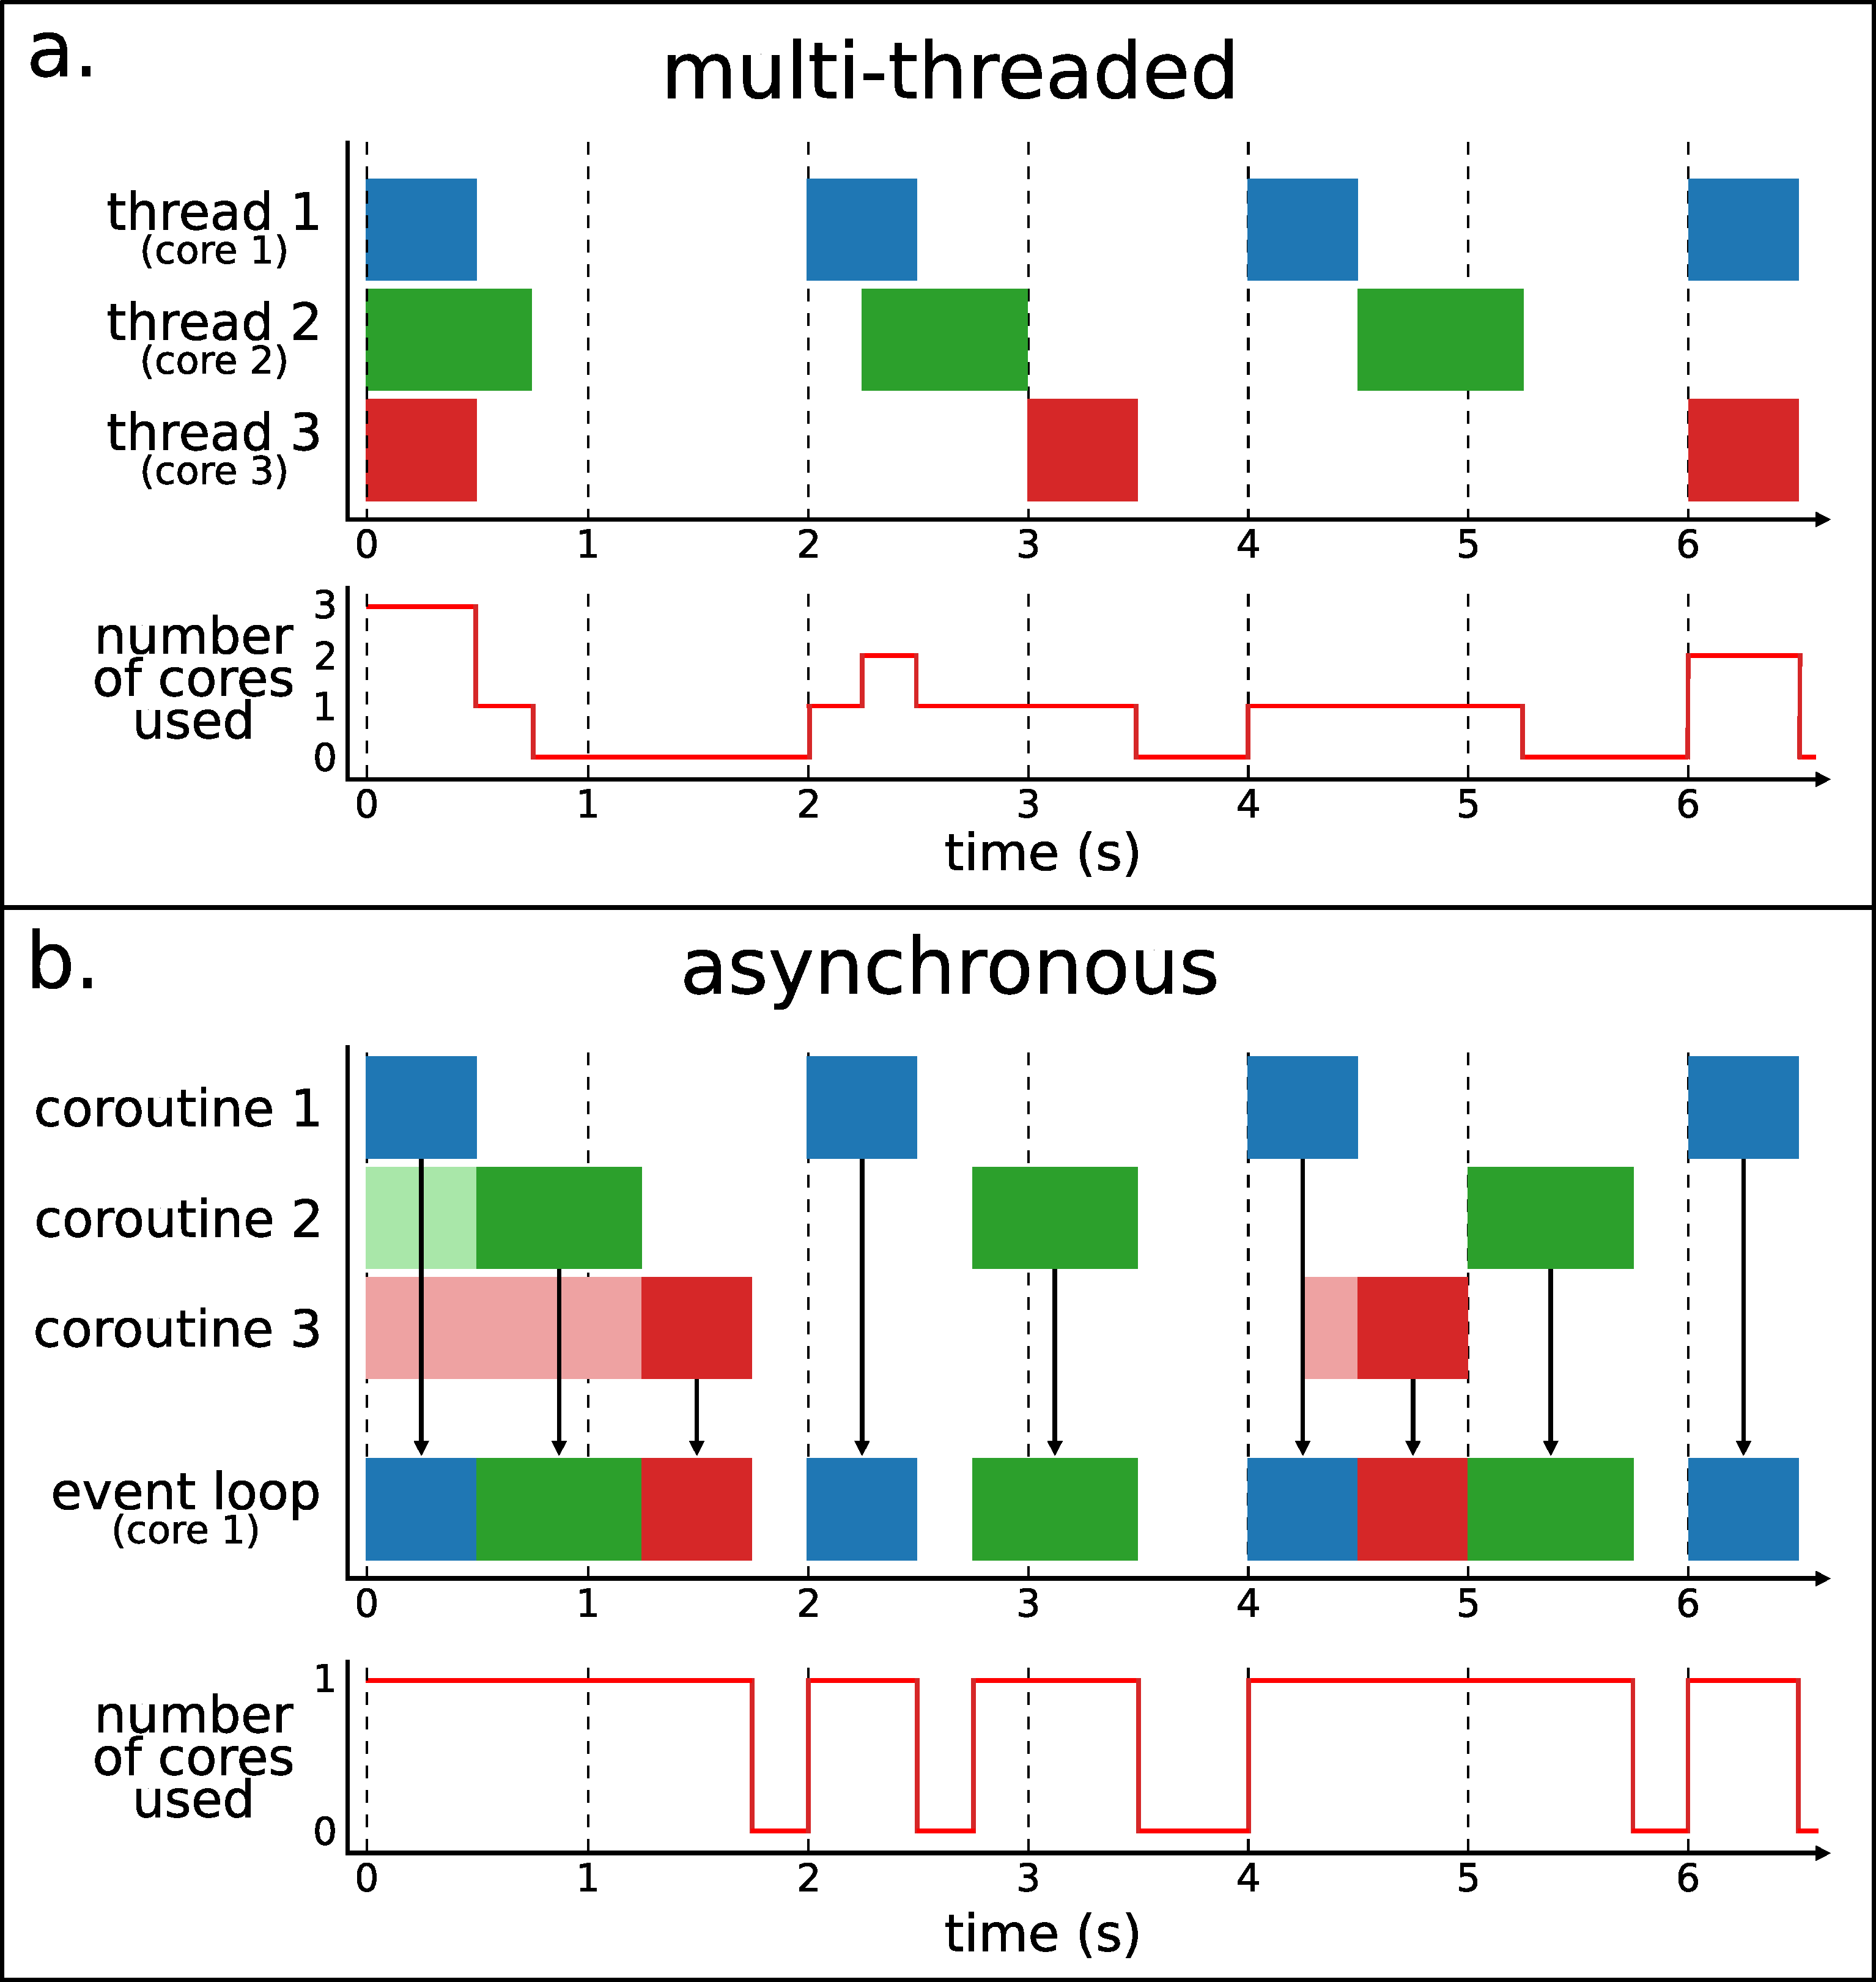
\includegraphics[width=0.9\linewidth]{images/async.pdf}
\end{center}
\caption[Multi-threaded vs asynchronous programming]{A comparison of multi-threaded vs asynchronous programming. This example uses a \textcolor{blue}{blue} task that takes \SI{0.5}{\second} to execute and then waits for \SI{1.5}{\second}, a \textcolor{ForestGreen}{green} task that takes \SI{0.75}{\second} and waits for \SI{1.5}{\second} and a \textcolor{red}{red} task that takes \SI{0.5}{\second} and waits for \SI{2.5}{\second}. These times are exaggerated for clarity, pilot tasks typically take less than a second and wait for between 10 and 60 seconds.
\\
\textbf{Top}: The three tasks with different execution periods (solid blocks) and wait times (blank) are run in a multi-threaded program. Each task is being run in an independent parallel thread on its own core, even though they rarely overlap and it is uncommon for multiple cores to be in use at the same time.
\\
\textbf{Bottom}: The same three tasks are run as coroutines in an asynchronous program. The event loop decides which coroutine to run on the single core, represented by the black arrows. This does lead to some coroutines being left waiting (lighter blocks) until the previous is finished, and as routines can be delayed it is not suitable for checks that need to happen at exact frequencies. However the overall core usage is much more efficient.}
\label{fig:async}
\end{figure}

% ---------
\subsubsection{The check routines}

The coroutines within the pilot can be separated into two types: the check routines and the night marshal. Most of the coroutines are designed as monitors to regularly check different parts of the system, which fits well into the asynchronous model. These check routines are as follows:

\begin{itemize}

\item \texttt{check\_flags} is a routine that monitors the system flags, most notably those created by the conditions daemon (see \aref{sec:conditions}). If any of the conditions flags are bad then the dome daemon will enter lockdown and close the dome on its own (see \aref{sec:dome}), but the \texttt{check\_flags} routine will abort exposures, pause the pilot and ensure it is not resumed until the flag is cleared. When the pilot is paused the dome will close, the mount will park, and the night marshal (see below) will not trigger any more tasks. When conditions are clear again the pilot will reopen the dome and allow normal operations to be restored. The \texttt{check\_flags} routine also monitors the system mode and will pause the pilot if it is set to manual mode or exit if set to engineering mode (see \aref{sec:mode}).

\item \texttt{check\_scheduler} is a routine that queries the scheduler daemon (see \aref{sec:scheduler}) every 10 seconds to find the best job to observe. If the pilot is currently observing the scheduler will either return the database ID of the current pointing, in which case the pilot will continue with the current job, or a new ID which will lead to the pilot interrupting the current job and moving to observe the new one. If the pilot is not currently observing (either it is the start of the night, resuming from being paused or the previous pointing has just completed) then it will begin observing whatever the scheduler returns. The details of how the scheduler decides which target to observe are given in \aref{sec:scheduler}. The ID returned is then passed to the observe (OBS) task run by the night marshal (see below).

\item \texttt{check\_hardware} monitors the hardware daemons (see \aref{sec:hardware_control}), checking every 60 seconds that they are all reporting their expected statuses. It does this using the hardware monitor functions, which are described below. If an abnormal status is returned then the pilot will pause and a series of pre-set recovery commands generated by the monitor are executed in turn. While in recovery mode the pilot will check the monitors more frequently. If the commands work and the status returns to normal the pilot is resumed, but if the commands are exhausted without the problem being fixed then an alert is issued that the system requires human intervention and the pilot triggers an emergency shutdown.

\item \texttt{check\_dome} is a backup to the primary hardware check routine. \texttt{check\_hardware} does monitor the dome along with the other hardware daemons, but \texttt{check\_dome} provides a simple, dedicated backup to ensure the dome is closed when it should be and to raise the alarm if it is not.

\end{itemize}

% ---------
\subsubsection{The hardware monitors}

One of the important tasks that the pilot is required to do is monitoring the status of the various system daemons, and therefore the hardware units they are connected to. If any problems were detected the easiest automated response would be to shutdown everything and send a message for a human to intervene. However this would be unnecessary in the case of small problems that could be easily fixed with one command, and it would be much better if the pilot could identify the problem and issue the command itself. The other benefit of this is a much faster reaction time than potentially needing to wake a human operator in the middle of the night, this is important both to minimise observing time lost and also potentially save the hardware by, for example, making sure the dome is closed in bad weather.

Therefore a system was created to enable the pilot to attempt to respond and fix any errors that occur itself. This is done within the \code{check\_hardware} coroutine though a series of hardware monitor \proglang{Python} classes, one for each of the daemons (i.e. \code{DomeMonitor}, \code{CamMonitor} etc.). Each daemon has a set of recognised statuses, representing the current hardware state, and a set of valid modes which represent the expected state. The current status is fetched from the hardware daemon, the mode is set by the pilot, and the hardware checks consist of comparing the two to discover if there are any inconsistencies. For example, the dome daemon can have current statuses of \code{OPEN}, \code{CLOSED} or \code{MOVING}, and its valid modes are just \code{OPEN} and \code{CLOSED}. At the start of the night when the pilot starts the dome should be in \code{CLOSED} mode, and the pilot only switches it to \code{OPEN} mode when it is ready to open the dome. If when a check is carried out the dome is in \code{CLOSED} mode but the current status is reported as not \code{CLOSED} then that is a problem, and the hardware check function returns that it has detected an error with the dome. These checks can have timeouts associated with each status. For example if the dome is in \code{CLOSED} mode and is reported as \code{MOVING} that is not necessarily an error, as it might be currently closing. The hardware monitor stores the time since the hardware status last changed, so if the dome reports that it has been in the moving state for longer than it would take to close then that raises an error. This example used states specific to that hardware, but every daemon also has various other possible states and errors --- for example if the daemon is not running, or is running and not responding.

When one of the monitor checks returns an error then the pilot will take action as described within the \code{check\_hardware} routine: pause night marshal (see below), stop any current tasks and send a Slack alert to record the error. But instead of stopping there, the monitor goes on to attempt to recover from the error and fix the problem. In the same way that a human observer would run though a series of commands in order to solve the problem, each monitor has a defined set of recovery steps to be run through depending on the error reported. Continuing with the previous example, if the dome reports \code{OPEN} when in \code{CLOSED} mode then the first recovery step is simple: execute the command \code{dome~open}. Each step then has a timeout value and an expected state if the recovery command worked. If after 10 seconds the status of the dome has not changed from \code{OPEN} to \code{MOVING}, then the error is persisting and more actions need to be taken. If however the dome daemon reports that the dome is moving then the error is not cleared immediately, only when the status finally reaches \code{CLOSED}. As mentioned previously, should a monitor run out of recovery steps then the pilot will send out an alert that there is nothing more that it can do and will attempt an emergency shutdown.

Using the above method, the vast majority of hardware issues can be solved by the pilot without the need for human intervention. Every time the recovery steps are triggered a message is sent to Slack detailing the error and the steps required to fix it, so it is easy to then go back and examine why the error occurred and how to prevent it in the future.

% ---------
\subsubsection{The night marshal}

The above check routines are support tasks for the primary routine, which is called the \texttt{night\_marshal}. Unlike the check routines the night marshal does not contain a loop, instead it runs through a list of tasks as the night progresses, based on the altitude of the Sun. Each task is contained in a separate \proglang{Python} observation script, which contains the commands to send to the hardware daemons. These scripts are self-contained programs which mean they can also be called independently, for example if the pilot is not running and a manual observer wants to run the autofocus routine they can use the command \texttt{obs\_script~autoFocus}. Each is run by spawning a new coroutine, meaning that while they are running the other routines such as the check tasks can continue. In the order they are performed during the night, the night marshal tasks are:

\begin{enumerate}

\item STARTUP, run immediately when the pilot starts. The \texttt{startup} script powers on the camera hardware, unparks the mount, homes the filter wheels and cools the CCDs down to their operating temperature of \SI{-20}{\celsius}. Once startup has finished the pilot will send a report of the current conditions to Slack (see \aref{fig:pilot_slack} below).

\item DARKS, run after the system start up is complete before opening the dome. This executes the \texttt{takeBiasesAndDarks} script to take bias and dark frames at the start of the night. \rtxt{see commissioning}

\item OPEN, run once the Sun reaches \SI{0}{\degree} altitude. It simply executes the \texttt{dome~open} command. If the pilot is paused due to bad weather or a hardware fault then the night marshal will wait and not open until the weather improves or fault is fixed. If it is never resolved then the night marshal will remain at this point until the end of the night and the shutdown timer runs out (see below).

\item FLATS, run once the dome is open and the Sun reaches \SI{-1}{\degree}. This executes the \texttt{takeFlats} script, which moves the telescope into a position pointing away from the Sun and then takes flat fields in each filter, stepping in position between each exposure and automatically increasing the exposure time as the sky darkens. See \aref{sec:flats} for details of the flat field routine.

\item FOCUS, run once the Sun reaches \SI{-11}{\degree}. This executes the \texttt{autoFocus} script, which finds the best focus position for each of the unit telescopes. See \aref{sec:autofocus} for details of the autofocus routine. If the routine fails for any reason the previous nights' focus positions are restored.

\item OBS (short for ``observing''), begun once the Sun reaches \SI{-15}{\degree} and continuing for the majority of the night until the Sun reaches \SI{-15}{\degree} again in the morning. When a database ID is received from the scheduler via the \texttt{check\_schedule} routine the \texttt{observe} script is executed. The script queries the observation database (see \aref{sec:obsdb}) to get the coordinates and exposure settings for that pointing and then sends the commands to the mount and exposure queue daemons. Once a job is finished, either through completing all of its exposures or being interrupted, the entry in the database is updated and the routine starts observing the next job from the scheduler.

\item FLATS is repeated once the Sun reaches \SI{-10}{\degree} in the morning, using the same script but this time increasing the exposure times as the sky brightens.

\end{enumerate}

% ---------
\subsubsection{Shutdown}

Once the night marshal has completed all of its tasks it exits and triggers the \texttt{shutdown} script, which powers off the cameras, parks the mount and ensures the dome is closed. Once this is finished the pilot quits. In addition there is a separate \code{night\_countdown} timer within the pilot, which will trigger the shutdown if the Sun ever reaches \SI{0}{\degree}. Normally the night marshal will have finished and triggered the shutdown long before that point, but the countdown acts as a backup ensuring that if there is a problem with the night marshal the pilot will still trigger a shutdown.

It is also possible for the pilot to trigger an emergency shutdown during the night. This triggers the same \texttt{shutdown} script observing script, with the only difference being that it ensures the dome is closed first. An emergency shutdown will be triggered by the pilot only in situations that it could not recover from without human intervention, notably if the \code{check\_hardware} routine reaches the end of a daemon's recovery steps without solving the problem.

% ---------
\subsubsection{The day marshal}

The day marshal is another script that provides a counterpart to the pilot (the mirror of the night marshal within the pilot). The \code{day\_marshal.py} script is run as a \software{cron} job like the pilot, but starts in the early morning rather than the late afternoon. The day marshal is a much simpler script, with only one key task --- to wait until dawn and then check that the dome is closed. In this sense it is yet another backup to the pilot's inbuilt \code{night\_countdown} timer, and as it is completely independent of the pilot it will run even if the pilot has crashed. Should it find that the dome is still open then the script will continuously try closing it, and send out human alerts that the system has failed. The day marshal will also send out a Slack report, again as a mirror of the report that the night marshal sends after startup, to confirm that the dome is closed.

% ---------
\subsubsection{\software{Slack} alerts}

Although the pilot is a completely robotic system it is still important that it doesn't operate completely unsupervised. As the \gls{goto} collaboration has adopted the \software{Slack} messaging client\footnote{\url{https://slack.com}} for instant messaging and collaboration it was decided that the telescope control system should send reports automatically to a dedicated Slack channel. This was implemented through the \proglang{Python} Slack \gls{api} module \pkg{slackclient}, and has been widely adopted throughout G-TeCS.\@ The two most complicated Slack messages are the startup report, sent by the night marshal within the pilot, and the morning report sent by the day marshal. The startup report includes a summary of the current condition flags, links to the site weather pages, the external webcam view and the latest IR satellite image over La Palma. The morning report includes the internal webcam view and plots showing what tiles the pilot observed last night and the current status of the all-sky survey. Examples of both are shown in \aref{fig:pilot_slack}. Several other functions send short reports, for example when the pilot starts and stops, when the dome opens and closes, if the system mode changes, or if a hardware error is being fixed. The pilot sends a majority of the messages to Slack but other daemons do as well, including the dome daemon when it enters lockdown (see \aref{sec:dome}) and the sentinel when it processes an interesting alert through GOTO-alert (see \aref{sec:sentinel}, \aref{sec:event_handling} and \aref{fig:gototile_slack}).

\begin{figure}[p]
    \begin{center}
    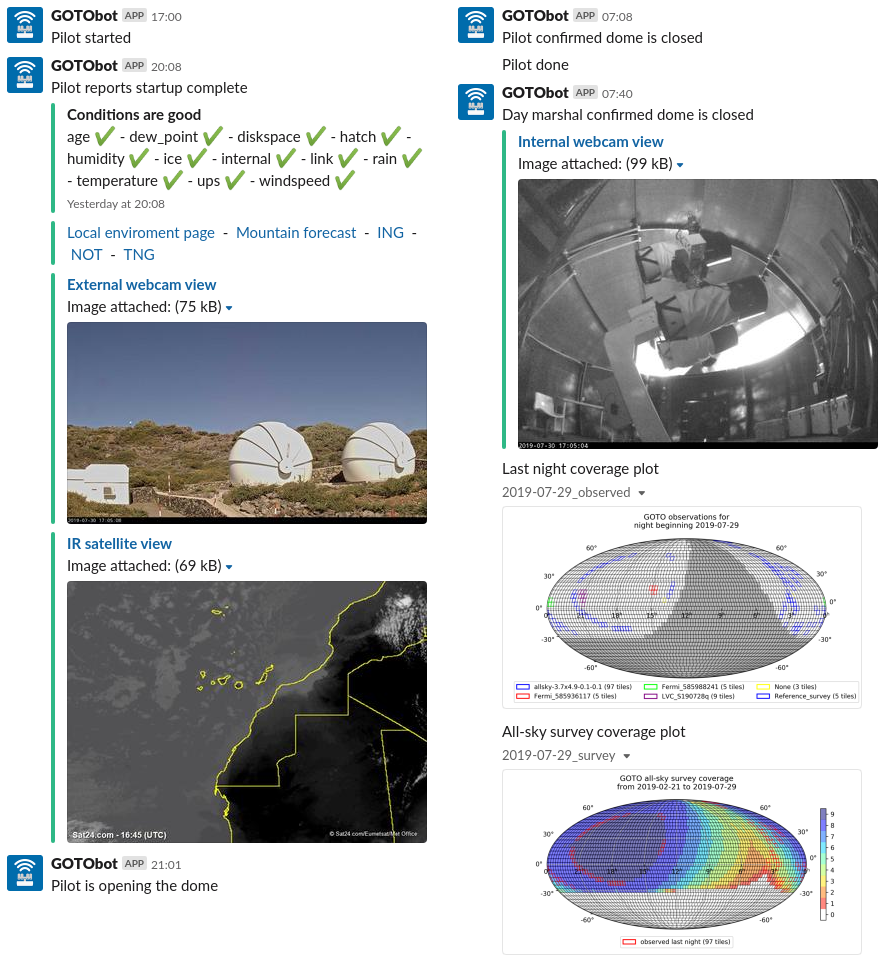
\includegraphics[width=\linewidth]{images/slack2.png}
    \end{center}
    \caption[Slack messages sent by the pilot and day marshal]{
        Slack messages sent by the pilot and day marshal on a typical night. The pilot reports when it starts automatically at 5pm, then the night marshal sends out the startup report when the STARTUP task has completed. The pilot also sends out messages when it is opening and closing the dome, and when it finishes in the morning. The day marshal later independently confirms the dome is closed and sends out its own morning report.
    }\label{fig:pilot_slack}
\end{figure}

\end{colsection}

% ~~~~~~~~~~~~~~~~~~~~

\newpage
\subsection{Conditions monitoring}
\label{sec:conditions}
\begin{colsection}

The conditions daemon is a support daemon that runs on the central observatory server in the SuperWASP building on La Palma (see \aref{fig:flow}). It takes in readings from the three local weather stations next to the GOTO dome on La Palma, as well as other sources such as internal sensors, every 10 seconds. The daemon processes these inputs into a series of output flags, which have a value of \code{0} (good), \code{1} (bad) or \code{2} (error). If any of the flags are marked as not good (i.e.\ the sum of all flags is $>0$) then the overall conditions are bad: the dome will enter lockdown and automatically close if it is open (see \aref{sec:dome}) and the pilot \code{check\_flags} routine will trigger the pilot to pause observations (see \aref{sec:pilot}). The conditions daemon is run on the central server because it deals with site-wide values, so when the second GOTO telescope on La Palma is built it is envisioned that they will both share the same conditions daemon (see \aref{sec:gtecs_multisite}).

Each conditions flag has a limit below or above which the flag will turn from good to bad. For categories with multiple sources (for example there are three local weather stations, located at GOTO, SuperWASP and W1m, and each gives an independent external temperature reading) then the limit will be applied to each and if \textit{any} are found to be bad then the flag is set. If follows therefore that \textit{all} the conditions sources must be good for the flag to be set to good. Each category also has two parameters, the bad delay and the good delay. These are the time the conditions daemon waits between an input going bad/good and setting the flag accordingly, which has the effect of smoothing out any sudden spikes in a value and ensures the dome will not be opening and closing too often.

The conditions flags can be grouped into three categories, divided according to severity. The latest version of G-TeCS contains 13 flags, listed in \aref{tab:conditions_flags}. An explanation of the different categories, and the flags within each, is given below.

\begin{table}[p]
    \begin{center}
        \begin{tabular}{c|cccc} % chktex 44
        Flag name           & Criteria measured & Bad criteria      & Good criteria     & Category    \\
        \midrule
        \code{dark}         & Sun altitude
                            & > \SI{0}{\degree}
                            & < \SI{0}{\degree}
                            & information
                            \\[20pt]

        \code{clouds}       & IR opacity
                            & > 40\%
                            & < 40\%
                            & information
                            \\[20pt]

        \code{rain}         & Rain detectors
                            & \makecell{\code{True} \\ for \SI{30}{\second}}
                            & \makecell{\code{False} \\ for \SI{10}{\minute}}
                            & normal
                            \\[20pt]

        \code{windspeed}    & Wind speed
                            & \makecell{> \SI{35}{\kilo\metre\per\hour} \\ for \SI{2}{\minute}}
                            & \makecell{< \SI{35}{\kilo\metre\per\hour} \\ for \SI{10}{\minute}}
                            & normal
                            \\[20pt]

        \code{humidity}     & Humidity
                            & \makecell{> 75\% \\ for \SI{2}{\minute}}
                            & \makecell{< 75\% \\ for \SI{10}{\minute}}
                            & normal
                            \\[20pt]

        \code{dew\_point}   & \makecell{Dew point \\ above ambient \\ temperature}
                            & \makecell{< +\SI{4}{\degree} \\ for \SI{2}{\minute}}
                            & \makecell{> +\SI{4}{\degree} \\ for \SI{10}{\minute}}
                            & normal
                            \\[20pt]

        \code{temperature}  & Temperature
                            & \makecell{< \SI{-2}{\degree} \\ for \SI{2}{\minute}}
                            & \makecell{> \SI{-2}{\degree} \\ for \SI{10}{\minute}}
                            & normal
                            \\[20pt]

        \code{ice}          & Temperature
                            & \makecell{< \SI{0}{\degree} \\ for \SI{12}{\hour}}
                            & \makecell{> \SI{0}{\degree} \\ for \SI{12}{\hour}}
                            & critical
                            \\[20pt]

        \code{internal}     & \makecell{Internal \\ temperature \\ \& humidity}
                            & \makecell{< \SI{-2}{\degree} or > 80\% \\ for \SI{1}{\minute}}
                            & \makecell{> \SI{-2}{\degree} and < 80\% \\ for \SI{10}{\minute}}
                            & critical
                            \\[30pt]

        \code{link}         & \makecell{Network \\ connection}
                            & \makecell{ping fail \\ for \SI{10}{\minute}}
                            & \makecell{ping okay \\ for \SI{1}{\minute}}
                            & critical
                            \\[20pt]

        \code{diskspace}    & \makecell{Free space \\ remaining}
                            & < 5\%
                            & > 5\%
                            & critical
                            \\[20pt]

        \code{ups}          & \makecell{Battery power \\ remaining}
                            & < 99\%
                            & > 99\%
                            & critical
                            \\[20pt]

        \code{hatch}        & Hatch sensor
                            & \makecell{\code{open} \\ for \SI{30}{\minute}}
                            & \makecell{\code{closed} \\ for \SI{30}{\minute}}
                            & critical
                            \\

        \end{tabular}
    \end{center}
    \caption[List of conditions flags and change criteria]{
        A list of all the conditions flags, and the criteria for them to switch from good to bad and bad to good.
        }\label{tab:conditions_flags}
\end{table}

\clearpage

The first category are the `information' flags. These are assigned values like the other flags, however they are purely for information purposes and do not contribute to the overall decision of whether the conditions are bad or not. In other words, an information flag can be bad, but the overall system conditions still considered good because the flag is not included in the final calculation. The information flag being being bad is not a reason to send the dome into lockdown, however it is still useful information to record. The two current information flags are described below:

\begin{itemize}
    \item \code{dark}: A simple information flag that is bad when the Sun is above the \SI{0}{\degree} horizon and good when it is below. This has no effect on the robotic system, but is useful for human observers.

    \item \code{clouds}: This information flag uses free IR satellite images downloaded from the \url{sat24.com} website to measure a rough cloud coverage value, based on the methods of \citet{clouds}. Although initially trialled as a normal flag, meaning the dome would close when high cloud was detected, the results were not consistent enough and the presence of clouds was more reliably calculated by the zero point measured by the data processing pipeline. The flag remains a useful information source however, and the satellite cloud opacity is added to the image headers to assist in later data quality control checks.
\end{itemize}

The second category contains the `normal' flags, and makes up the conditions flags relating to the external weather conditions. These flags going bad are valid grounds to close the dome, however as they relate to natural events they are not in any way unusual and the pilot can happily remain paused and wait for the flags to clear. The normal flags are described below:

\begin{itemize}
    \item \code{rain}: This flag is set to bad if any of the weather stations report rain, and will only be cleared after 10 minutes of no more rain being reported. In practice rain usually coincides with high humidity, meaning the \code{rain} and \code{humidity} flags often overlap.

    \item \code{windspeed}: This flag gets set if the windspeed is above \SI{35}{\kilo\meter\per\hour}, with a bad delay of two minutes and a good delay of ten minutes. The wind limit was previously \SI{40}{\kilo\metre\per\hour} but when the full four unit telescope array was installed, with the addition of the light shields, the wind sensitivity of the mount was increased and the high wind limit had to be lowered.

    \item \code{humidity} The humidity limit is 75\%, with a bad delay of two minutes and a good delay of ten minutes.

    \item \code{dew\_point}: The dew point is related to the humidity, and has a limit of \SI{4}{\celsius} above the ambient external temperature (so if the external temperature is \SI{20}{\celsius} then the flag is set to bad if the dew point is \SI{24}{\celsius} or below).

    \item \code{temperature}: The \code{temperature} flag is set if the temperature drops below \SI{-2}{\celsius} for two minutes, and also has a good delay of ten minutes. The telescope can operate in below-freezing temperatures for short amounts of time, but for longer cold periods when ice build-up is a concern see the critical \code{ice} flag below.

\end{itemize}

The final category are the `critical' flags, for more serious situations that might arise. In early versions of G-TeCS any of these flags turning bad was enough to trigger an emergency shutdown and stop the pilot for the night. However this proved to be an over-reaction and there were no issues with having the pilot continue, although remaining paused while the flag was bad. The only difference now between `normal' and `critical' flags is that when a critical flag turns bad a Slack alert is sent out to ensure it is brought to the attention of the human monitors. The critical flags are described below:

\begin{itemize}
    \item \code{ice}: A critical flag which uses the same input as the \code{temperature} flag, but is set to bad if the temperature is below \SI{0}{\celsius} for 12 hours and will only clear if it is constantly above freezing for another 12 hours. These longer timers mean this flag prevents the dome opening after a serious cold period until the temperature is regularly back above freezing, and also gives time for a manual inspection to be carried out to ensure the dome is free of ice.

    \item \code{internal}: A combination flag for the two internal temperature and humidity sensors within the dome. These have very extreme limits, a humidity of above 80\% or a temperature of below \SI{-2}{\celsius}, which should never be reached inside under normal circumstances due to the internal dehumidifier. This flag therefore is a backup for an emergency case, when either the dehumidifier is not working or the dome has somehow opened in bad conditions.

    \item \code{link}: The conditions daemon also monitors the external internet link to the site, by pinging the Warwick server and other public internet sites. After 10 minutes of unsuccessful pings the flag is set to bad. It is technically possible for the system to observe without an internet link, and there is a backdoor into the system through the SuperWASP network, but it is an unnecessary risk: in an emergency alerts could not be sent out and external users would not be able to log in.

    \item \code{diskspace}: The amount of free disk space on the image data drive is also monitored, with the flag being set to bad if there is less than 5\% of free space available. As images are immediately sent to Warwick and then regularly cleared from the local disk this should never be an issue, but this is a critical conditions flag as if the local disk was full it would prevent any more data being taken.

    \item \code{ups}: The conditions daemon will set the \code{ups} flag if the observatory has lost power and the system UPSs are discharging (see \aref{sec:power}). Brief power cuts do occur on La Palma, but rarely for more than a few minutes as there are on-site backup generators that take over.

    \item \code{hatch}: A critical flag to detect if the access hatch into the dome has been left open. This flag is unique in that is is only valid in robotic mode (see \aref{sec:mode}); when in manual or engineering mode it is assumed that the hatch being opened is a result of someone operating the telescope. But when the system is observing robotically the hatch being open is a problem, as there is no way to close it remotely and in bad weather damage could be caused to the telescope.
\end{itemize}

\end{colsection}

% ~~~~~~~~~~~~~~~~~~~~

\subsection{The observation database}
\label{sec:obsdb}
% Time Blocks??
\begin{colsection}

The scheduling system for \gls{gtecs} is based around a database known as the observation database or ``ObsDB''. This database is located on the central observatory server hosted by SuperWASP, which not only is a faster machine than the control computer in the dome but in the future will allow a single database to be shared between mounts (see \aref{sec:gtecs_multisite}). The database is implemented using the \software{MariaDB} database management system\footnote{\url{https://mariadb.com/}}, an open-source fork of the established \software{MySQL} system, and is queried and modified using \gls{sql} commands. In order to interact easily with the database within G-TeCS code a separate \software{Python} module, \pkg{obsdb}, was written as an \gls{orm} package utilising the existing \pkg{sqlalchemy} module\footnote{\url{https://sqlalchemy.org/}}.

The primary table in the database is for individual \textit{pointings}. These each represent a single visit of the telescope, with defined RA and Dec coordinates and a valid time range for it to be observed within, as well as other observing constraints. Each pointing has a status value which is either \code{pending}, \code{running}, \code{completed} or some other terminal status (\code{aborted}, \code{interrupted}, \code{expired} or \code{deleted}). Ideally a pointing passes through three stages: it is created as \code{pending}, the scheduler selects it and the pilot marks it as \code{running}, then if all is well when it is finished it is marked as \code{completed}. If it stays in the database and never gets observed it will eventually pass its defined stop time (if it has one) and will be marked as \code{expired} by the database caretaker script. If the pointing is in the middle of being observed but is then cancelled before being completed it will be marked either \code{interrupted} (if the scheduler decided to observe another pointing of a higher priority) or \code{aborted} (in the case of a problem such as having to close for bad weather). The \code{deleted} status is reserved for pointings being removed from the queue before being observed, such as updated pointings being inserted by the sentinel and overwriting the previous ones (see \aref{sec:db_insert}). A representation of the relationship between the pointing statuses and how they progress is shown in \aref{fig:pointings}.

\begin{figure}[p]
    \begin{center}
        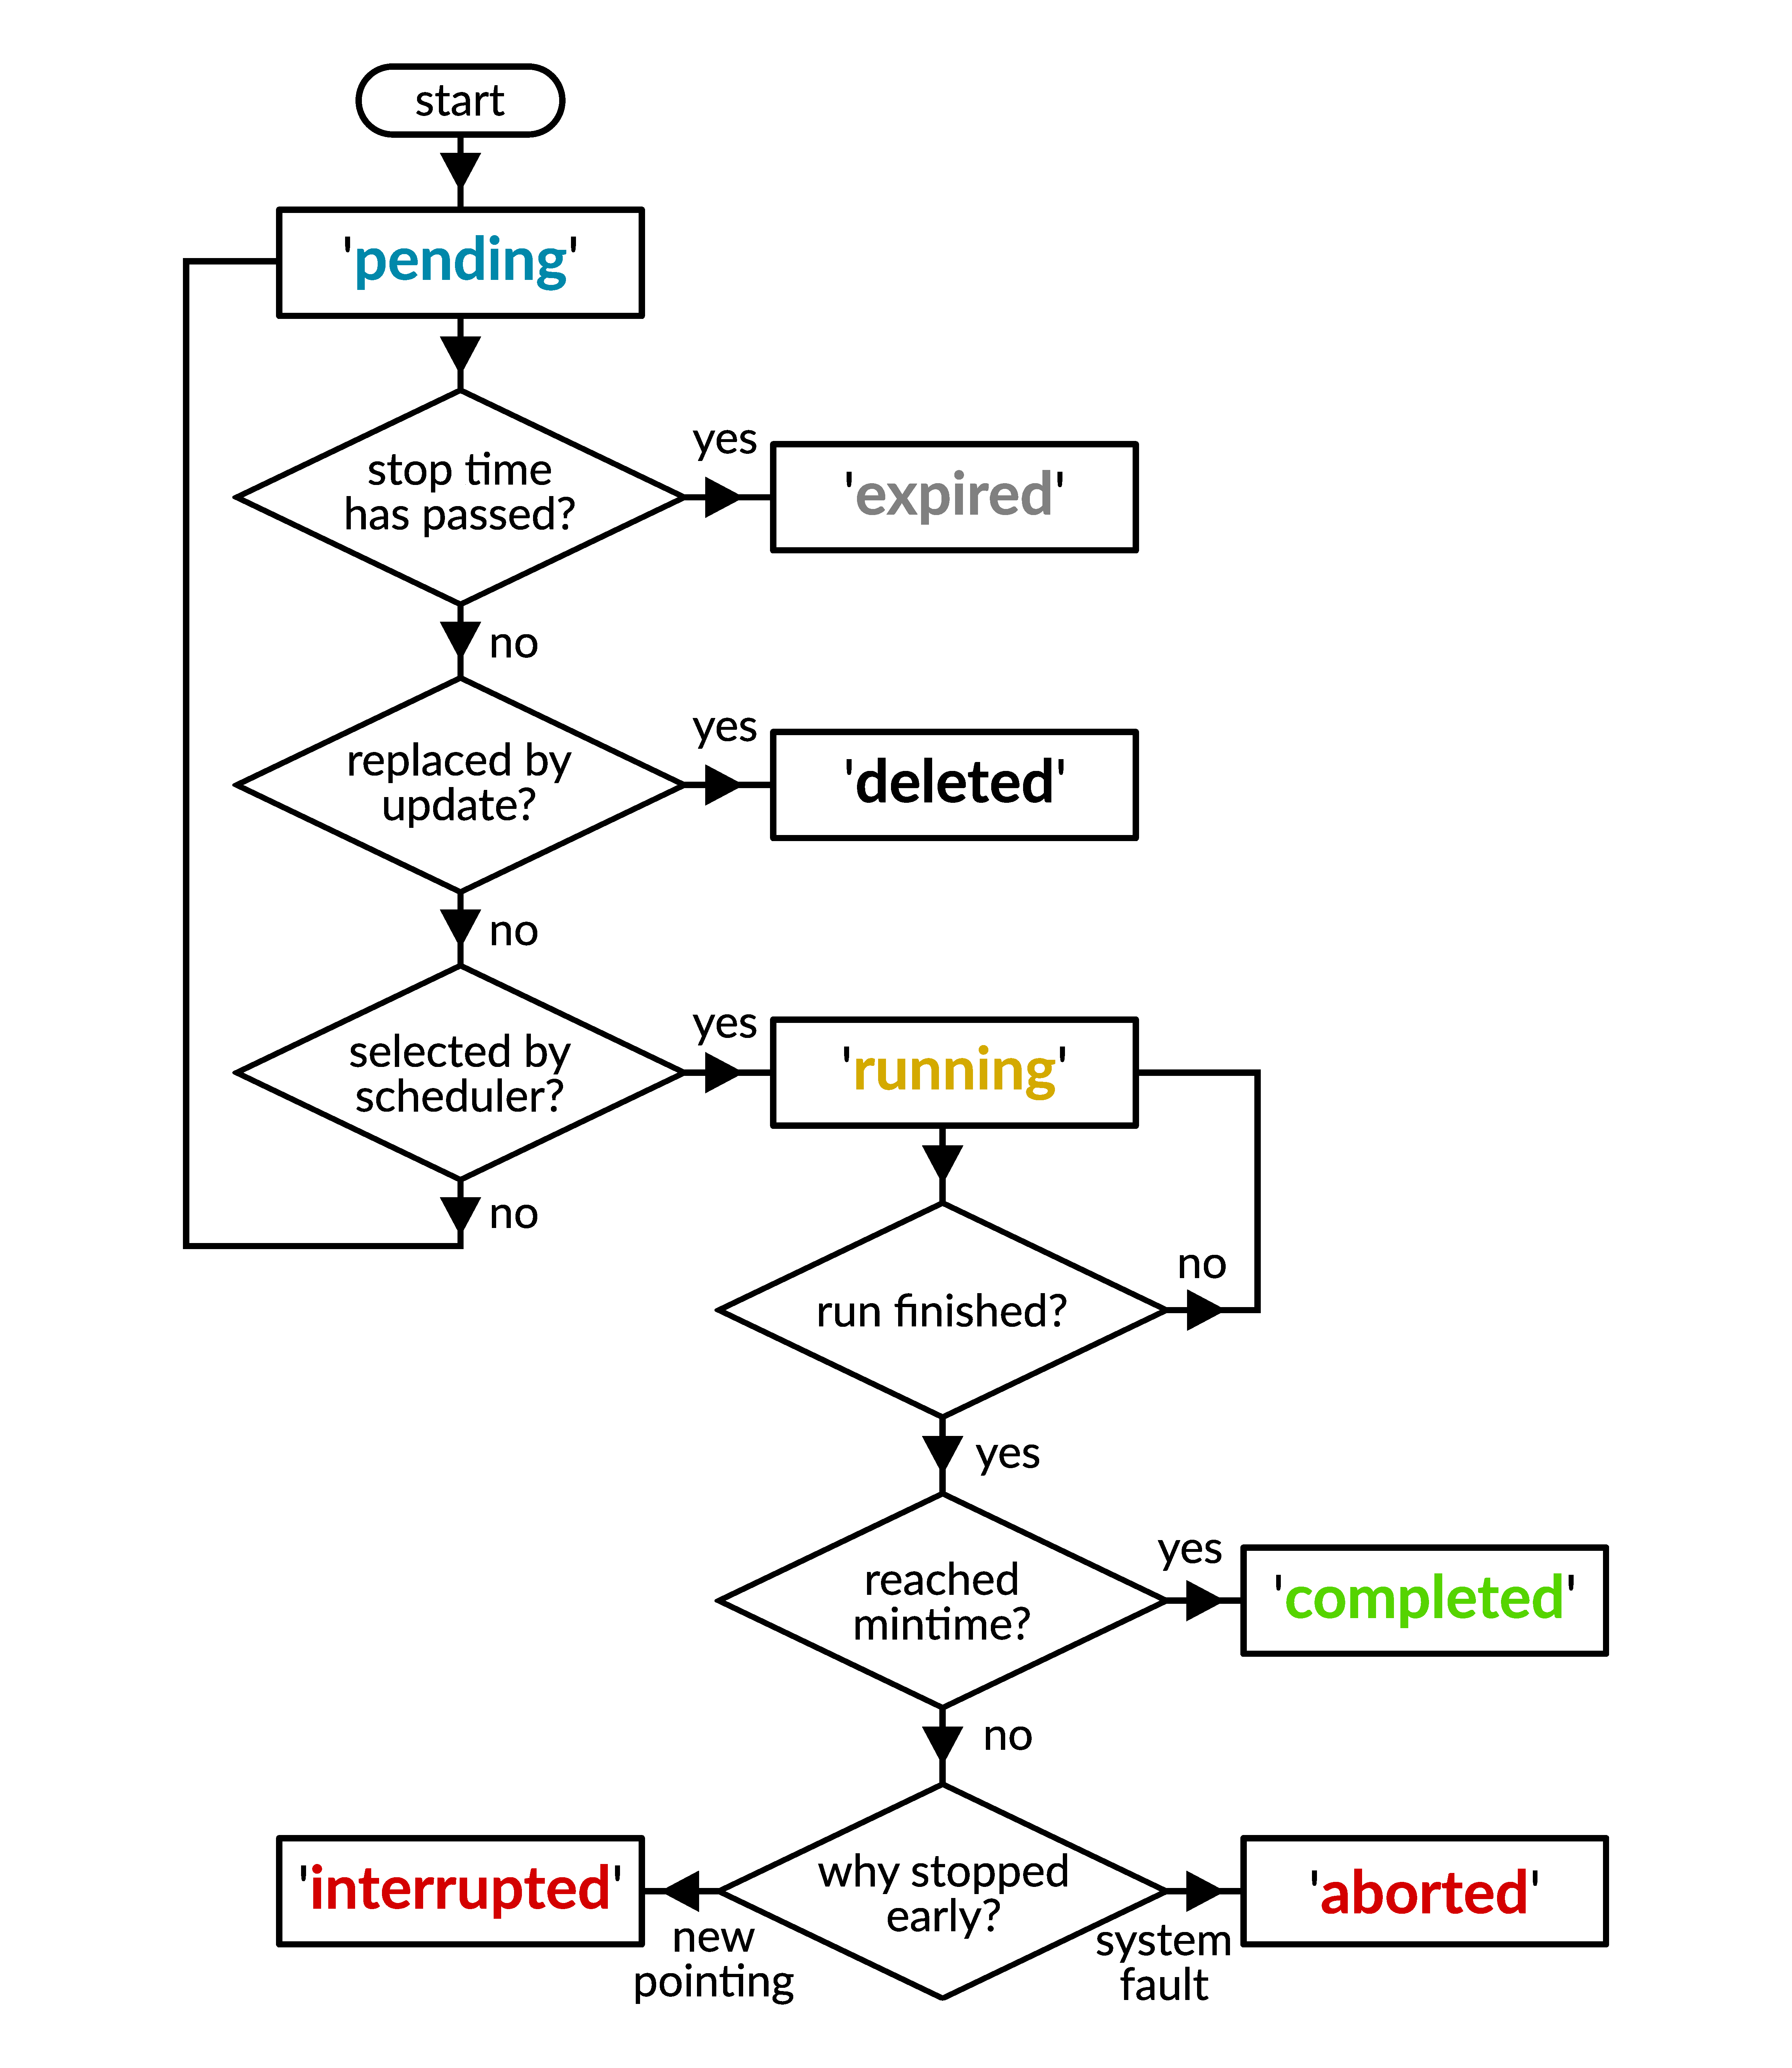
\includegraphics[width=0.9\linewidth]{images/pointings_flowchart.pdf}
    \end{center}
    \caption[Pointing status progression flowchart]{
        A flowchart showing how the status of an entry in the pointings table can change.
        }\label{fig:pointings}
\end{figure}

\clearpage

As well as the target information (RA, Dec, name) a pointing entry contains constraints on when they can be observed. Each pointing can have set start and stop times; the scheduler will only select pointings where the current time is within their valid range (and once the stop time has passed they will be marked as \code{expired}). Limits can also be set on minimum target altitude, minimum distance from the Moon, maximum Moon brightness (in terms of Bright/Grey/Dark time) and maximum Sun altitude. These constraints are applied by the scheduler to each pointing when deciding which to observe, and unless they all pass the pointing is deemed invalid (see \aref{sec:scheduler}). When created, a pointing is also assigned a rank, usually from 0--9, as well as a True/False flag marking it as a time-critical Target of Opportunity (ToO). These are used when calculating the priority of the pointing, to compare with others in order to determine which is the highest priority to observe.

The commands to be executed once the telescope has slewed to a pointing are stored in a separate \code{exposure\_sets} table. An exposure set defines what commands the pilot will give to the exposure queue daemon (see \aref{sec:exq}). The table has columns for the number of exposures to take, the exposure time and the filter to use. For example an observation requiring three \SI{60}{\second} exposures in the L filter followed by one each in the R, G and B filters would require four entries in the table: each with exposure time of \SI{60}{\second}, the first with number of exposures as 3 and filter as L and the rest with number of exposures as 1 and the individual filters. When the pointing is observed by the pilot will add the linked exposure sets to the queue, and each will then be observed in turn.

Each entry in the pointings table can only be observed once. For observing a target more than once there also exists the \code{mpointings} table, which contains information to dynamically re-generate pointings for a given target. An mpointing entry is defined with three key values: the requested number of observations, the time each should be valid in the queue and the time to wait between each observation. Each time the database caretaker script is run it looks for any entries in the mpointing table that still have observations to do and it creates another entry in the pointings table for that target. Setting the time values allows a lot of control over when pointings can be valid, for example scheduling follow-up observations a set number of hours or days after an initial pointing is observed.

The three tables described above (\code{pointings}, \code{exposure\_sets} and \code{mpointings}) are the core tables required for observation scheduling. However there are other tables defined in the database which are used to group pointings together and relate to GOTO's purpose as a survey instrument. As described in more detail in \aref{sec:gototile}, GOTO observes the sky divided into a fixed grid of individual tiles. The database therefore also contains a \code{grids} table and a \code{grid\_tiles} table, which define the current grid based on the field of view of the telescope. Mapping pointings to the grid is achieved through two more tables, \code{surveys} and \code{survey\_tiles}. A \textit{survey} in this context is a group of tiles that are being observed for a specific reason, one example are the pointings comprising the all-sky survey that \gls{goto} carries out every night. Events that are processed by the alert sentinel (see \aref{sec:sentinel}) might have a skymap that covers multiple tiles, and therefore the set of pointings required to cover it forms a survey within the database. Each pointing within the survey is linked to a survey tile, and each survey tile is linked to a grid tile of the current grid. The additional field added by the survey tile is a `weighting' column, which allows tiles within a survey to be weighted relative to each other. In the all-sky survey each tile is weighted equally, but in a survey coming from an event skymap the tiles will be weighted by the contained probability within that tile. The scheduler takes this weighting into account when deciding which pointing to observe (see \aref{sec:scheduler}, and \aref{sec:scheduler_sims} for more details).

There are two additional tables that are used to contain supporting information: the \code{events} and \code{users} tables. The \code{events} table contains fields such as the event type and source, and is filled by the sentinel when events are processed (see \aref{sec:sentinel}). The \code{users} table connects each pointing to the user who added it to the database. At the moment this is unused, and each pointing is linked to the single generic ``GOTO'' user, but in the future individuals might wish to insert and keep track of their own targets.

\end{colsection}

% ~~~~~~~~~~~~~~~~~~~~

\subsection{The sentinel}
\label{sec:sentinel}
\begin{colsection}

In order for targets to be observed by GOTO in robotic mode they must have entries defined in the \code{pointings} table in the observation database (see \aref{sec:obsdb}). These can be added manually, but for automated observation they have to be inserted whenever an alert is detected. This is the job of the sentinel daemon, as shown in \aref{fig:flow}.

In addition the normal control loop, the sentinel daemon includes an independent alert listener loop that is continuously monitoring the transient alert stream outputted by the 4 Pi Sky event broker \citep{4pisky}, using functions from the \pkg{pygcn} \proglang{Python} package\footnote{\url{https://pypi.org/project/pygcn/}}. Should the link to the 4 Pi Sky server fail then the daemon will automatically attempt to re-establish the connection every few seconds until it is restored. Alerts come in to the listener in the form of VOEvents \citep{voevent}, and pending alerts are appended to an internal queue before being processed using the event handler defined in the \proglang{Python} module GOTO-alert (\pkg{gotoalert}, see \aref{sec:event_handling}). The sentinel also has an additional \code{ingest} command which can be used to manually insert test events or bypass the alert listener. The details of how alerts are processed are described in \aref{chap:events}, which includes \aref{sec:gototile} discussing how HEALPix probability skymaps are mapped onto the GOTO all-sky grid and \aref{sec:gotoalert} detailing how VOEvents are processed and added to the database.

The alert listener is a key part of the automated system but was not initially planned to be assigned to its own independent daemon. The \gls{pt5m} system uses the \software{Comet} software \citep{comet} in a separate script independent of any daemons. The advantages to including a dedicated alert listener daemon in G-TeCS, which became known as the sentinel, come from it being integrated into the pilot monitoring systems like the other daemons (described in \aref{sec:pilot}). Should the sentinel daemon crash or not respond to checks the pilot will notice and restart it like any other daemon.

\end{colsection}

% ~~~~~~~~~~~~~~~~~~~~

\subsection{The scheduler}
\label{sec:scheduler}
\begin{colsection}

In order for a target to be observed by the telescope in robotic mode an appropriate pointing must be added to the observation database (or an ``mpointing'' entry that generates pointings, as described in \aref{sec:obsdb}). These can be added manually if desired, but in most cases they are either defined once when the database is created (for the constant all-sky survey tiles) or added by the sentinel daemon when a transient alert is received. All entries in the \code{pointings} table with status ``\code{pending}'' form the current \textit{queue}, and the task of selecting which of these pointings the system should observe is the role of the scheduler.

% ---------
\subsubsection{The scheduler daemon}

Within \gls{gtecs} the \textit{scheduler} can refer to two linked concepts: the scheduling functions or the scheduler daemon itself (which is often just called ``the'' scheduler, like the sentinel). In the \gls{pt5m} system there is no independent ``scheduler'' daemon, and when the pilot needs to know what to observe it simply calls the scheduling functions to read the current queue, rank the pointings and find the one with the highest priority. When expanding the system for \gls{goto} it was decided to farm these calculations off to a separate daemon, which the pilot instead queries just like the other hardware daemons. There are several advantages to this method. Firstly the scheduling commands can take a significant amount of time (several seconds), so splitting this out to a separate program saves time and frees up the pilot thread for other routines (recall the pilot is asynchronous but not multi-threaded). Secondly separating out the scheduling to an independent daemon allows it to be run on a different computer to the pilot. As shown in \aref{fig:flow} the scheduler daemon runs on the same central server in SuperWASP that hosts the observing database (see \aref{sec:obsdb}), which improves the speed of the database queries. The central server is also simply a more powerful machine than the NUC in the dome that runs the pilot and other hardware daemons, which also reduces the time to run the queries. Finally, when GOTO moves to a multi-telescope system it is anticipated that the scheduler will be one of the common systems shared between telescopes (see \aref{sec:gtecs_multisite}), and so it makes sense to have the scheduler daemon on the central server alongside the other shared systems.

The scheduler daemon contains the usual control loop, which runs the scheduling functions described below and internally stores the returned highest-priority pointing. The daemon exposes a single command, \code{check\_queue}, which returns the ID of that pointing. The pilot \code{check\_schedule} coroutine queries the daemon every 10 seconds using this command, and the scheduler returns one of three results: carry on with the current observation, switch to a new observation, or park the telescope (in the case that there are no valid targets). Most of the time the pilot will be observing a pointing previously given by the scheduler, and on the next check the scheduler will return the same pointing as it is still the highest priority --- in which case pilot will continue observing it. Even if the scheduler finds that a different pointing now has a higher priority it will not tell the pilot to change targets whilst observing the current target, unless the new pointing has the \glsfirst{too} flag set. Otherwise the pilot will wait until it has finished the current job, mark it as complete in the database and ask the scheduler for the next target to observe. The different cases are summarised in \aref{tab:sched}.

%\begin{landscape}
%\begin{table}[p]

\begin{sidewaystable}[p]
    \begin{center}
        \begin{tabular}{cc|cccc} % chktex 44
            &
            & \multicolumn{4}{c}{Highest priority pointing is\ldots}
            \\[0.5cm]

            &
            & \makecell{\ldots same as \\ current pointing}
            & \makecell{\ldots a new, \\ valid pointing}
            & \makecell{\ldots a new, \\ invalid pointing}
            & \ldots None
            \\[0.5cm]

            \midrule
            & & & & &
            \\

            \multirow{8}{*}{\rotatebox[origin=c]{90}{Current pointing is\ldots}}
            & \ldots valid
            & \makecell{\textcolor{ForestGreen}{Continue} \\ \textcolor{ForestGreen}{current pointing}}
            & \makecell{\textcolor{BlueGreen}{Interrupt and start new pointing} \\ \textcolor{BlueGreen}{if it is a ToO and the current pointing is not,} \\ \textcolor{BlueGreen}{otherwise continue current pointing}}
            & \textcolor{red}{Park}
            & \textcolor{red}{Park}
            \\[1.5cm]

            & \ldots invalid
            & \textcolor{red}{Park}
            & \textcolor{NavyBlue}{Interrupt and start new pointing}
            & \textcolor{red}{Park}
            & \textcolor{red}{Park}
            \\[1.5cm]

            & \ldots N/A (parked)
            & \textcolor{red}{Remain parked}
            & \textcolor{NavyBlue}{Unpark and start new pointing}
            & \textcolor{red}{Remain parked}
            & \textcolor{red}{Remain parked}
            \\[0.5cm]

        \end{tabular}
    \end{center}
    \caption[Actions to take based on scheduler results]{
        Actions the pilot will take based on the scheduler results. The scheduler can return one of three options as the highest priority pointing: the current pointing, a different pointing or \code{None} (meaning the current queue is empty). Each pointing can either be valid or invalid. The pilot will either continue with the current pointing (\textcolor{ForestGreen}{green}), switch to the new pointing depending on the ToO flag (\textcolor{NavyBlue}{blue}, \textcolor{BlueGreen}{blue-green}) or park the telescope (\textcolor{red}{red}).
    }\label{tab:sched}
\end{sidewaystable}

%\end{table}
%\end{landscape}

\newpage
% ---------
\subsubsection{Determining the highest priority target}

\gls{goto} operates under a ``just-in-time'' scheduling model \citep[see, for example,][]{LCO_scheduling}, rather than creating a fixed plan at the beginning of the night of what to observe \citep[see, for example,][]{ZTF_scheduler}. Each time the pilot queries the scheduler the current queue of pointings is imported and the priority of each is calculated, with no explicit consideration for the past or future (aside from the ``mintime'' constraints, as described below). The highest priority pointing is then returned to the pilot, as described above. This system is very reactive to any incoming alerts as the new pointings will immediately be included in the queue at the next check. This method also naturally works around any delay in observations due to poor conditions, which a fixed night plan can not do. The just-in-time method can be less efficient than a night plan when observing predefined targets which can be deliberately optimised before the night starts. However the just-in-time system is perfectly reasonable for the all-sky survey GOTO is normally observing, and any other observations will be alerts entered by the sentinel daemon which could not be planned for. Hence a ``just-in-time'' scheduler is the best option for GOTO.\@

Each time the scheduler is called several steps need to be carried out. The first of these is to fetch the current queue from the observation database. This is done by querying the database \code{pointings} table for any entries that have the \code{pending} status. Additional filters are also applied in order to reduce the number of invalid pointings imported: restricting the query to pointings within the visible region of the sky (based on the time and observatory location) and within the pointing's valid period (the start time has passed and stop time has not yet been reached). Any entries in the pointings table that pass these filters make up the queue of pointings passed to the scheduler.

In order to find which pointing is the highest priority the queue is sorted using a variety of parameters, with the pointing sorted at the top being returned by the scheduler. The sorting criteria are outlined below.

\newpage

The first consideration is determining which pointings are currently valid. As described in \aref{sec:obsdb}, pointings have limits defined for physical constraints (minimum altitude, minimum Moon separation, maximum Moon illumination, maximum Sun altitude). These constraints are calculated and applied to the pointings using the \pkg{astroplan} \proglang{Python} module \citep{astroplan}. All of the constraints depend on the current time and three of the four on the current position of the target in the sky (the Moon illumination is independent of the target). These constants are applied both at the current time and after each pointing's minimum time. This ensures that, for example, targets that are setting are visible throughout their observing period by checking the altitude is above the minimum both at the beginning and end of the observation. The minimum time constraints are not applied to the pointing currently being observed (if any), as the pointing will already be part way through and will have already been passed as valid. The validity of the pointings is a simple boolean flag (True or False), and invalid pointings are sorted below valid ones.

The next order pointings are sorted by is the effective rank of the pointing, which is a combination of the integer starting rank the pointing was inserted with and the number of times it has been observed.

The starting rank is fixed when the pointing is created: every pointing is given an integer rank between 0 and 999, with highest and lowest ranks being reserved for particular classes of targets. Rank 0 is not intended to be used under normal circumstances: it is reserved for exceptional events, such as a local galactic supernova, as a pointing with rank 0 would outrank all other pointings including even gravitational wave events. At the other end of the scale, rank 999 is reserved for the all-sky survey tiles so they are sorted below all other pointings. These pointings act as ``queue fillers'' in the system, ensuring there is always something for the telescope to observe. All other ranks are otherwise available, although by convention ranks ending in 1--5 are used for gravitational wave events, 6--8 for other transient events (e.g. GRBs) and 9 for other fixed targets. See \aref{sec:event_strategy} for the details of determining the rank for different transient events.

Added to the starting rank is a count of the number of times that a target has been observed, based on the number of pointings previously associated with a given mpointing (see \aref{sec:obsdb}). This count only includes successful observations, so pointings that were interrupted or aborted are not included. The starting rank ($R_s$) and observation count ($n_\text{obs}$) are added to create the effective rank $R$ given by

\begin{equation}
    R = R_s + 10\times n_\text{obs}.
    \label{eq:effective_rank}
\end{equation}

This formula means a pointing with a starting rank of 2 that has been observed five times will have an effective rank of 52. Effective ranks are sorted in reverse order, so a rank-5 pointing that has been observed once (an effective rank of 15) will be a higher priority target than a rank-4 pointing that has been observed twice (an effective rank of 24). This system allows for a natural filtering of targets, as targets will move down the queue as they are observed. For example, pointings from a gravitational wave event might be inserted into the database at rank 2, so will first appear in the queue with effective rank of $R=2$ ($n_\text{obs}=0$). The first pointing that is observed will reappear with $R=12$, and therefore be sorted below those tiles that have not yet been observed. Once all the pointings have been observed once they will all have effective rank 12 and the process repeats, with each pointing falling to effective rank 22, 32 etc. As the increase is by 10 each time pointings from other events or which were manually inserted might also be in the queue and interweave between the event follow-up pointings. For example, a manual observation might be inserted at rank 9, meaning it will fall below the first observation of the gravitational wave tiles at $R=2$ but will take priority over subsequent observations. To prevent this, the manual observation could be inserted at rank 19 to come after two GW observations, or even 509 to completely ensure it does not interfere with the gravitational wave follow-up targets.

For pointings with the same effective rank the next sorting parameter is the \glsfirst{too} flag assigned to the pointing when it was inserted into the database. The flag is simply a boolean value that is true if the target is a ToO and false if it is not, and pointings that have the flag as true are sorted higher than those of the same rank that are not ToOs. This ensures that time-sensitive targets come ahead of other targets at the same rank, although it is important to remember that the effective rank does still take priority (so a ToO at rank 4 will be a lower priority than a non-ToO at rank 3).

Finally, should all the above parameters still result in multiple pointings with the same priority, a final tie-break value calculated for each pointing. This value is based on the current airmass of the pointing and the weighting of the survey tile the pointing is linked to, if any. Pointings at lower airmass (closer to the zenith) and higher tile weightings are given the higher priority. To calculate the tiebreak both parameters need to be scaled between 0 and 1. Tile weights are usually already in percent, while the airmass is inverted and scaled so airmasses 1 and 2 are set to 1 and 0 respectively (airmasses greater than 2 are set to zero). The weighting ($W$) and airmass ($X$) values are then combined to form the tiebreak value $T$ in a ratio 10:1, so the final tiebreak value is given by

\begin{equation}
    T = \frac{10}{11} \times W + \frac{1}{11} \times (2 - X)
    \label{eq:tiebreak}
\end{equation}

This ensures the tiebreak value $T$ is also between 0 and 1, with higher values being preferred. The best possible scenario is a tile which contains 100\% of the probability ($W=1$) and is exactly at zenith ($X=1$) which gives a tiebreak value $T=1$. The 10:1 ratio was determined based on scheduler simulations detailed in \aref{sec:scheduler_sims}, and the above \aref{eq:tiebreak} is a simplification of \aref{eq:pat}.

In the unlikely event that two pointings are still tied, all other parameters being otherwise equal and they have the same tiebreak value, then whichever was inserted into the database first (and therefore has a lower database ID) by default comes first in the queue.

\newpage

%% Tiebreaker is calculated with
%% =((2-<airmass>)*0.1+<prob>*0.9)

\begin{table}[t]
    \begin{center}
        \begin{tabular}{c|l|c|rrr|c|ccc} % chktex 44
            & Name & Valid & $R_s$ & $n_\text{obs}$ & $R$ & ToO & Airmass & Tile weight & Tiebreaker
            \\
            \midrule
            1 &
            GW 191202 P3 &
            \textcolor{Green}{Y} &
            \textcolor{Blue}{2} &
            \textcolor{Orange}{0} &
            2 &
            \textcolor{Green}{Y} &
            1.1 &
            0.10 &
            0.180 \\

            2 &
            GW 191202 P4 &
            \textcolor{Green}{Y} &
            \textcolor{Blue}{2} &
            \textcolor{Orange}{0} &
            2 &
            \textcolor{Green}{Y} &
            1.1 &
            0.05 &
            0.135 \\

            3 &
            M101 &
            \textcolor{Green}{Y} &
            \textcolor{Blue}{9} &
            \textcolor{Orange}{0} &
            9 &
            \textcolor{Red}{N} &
            1.5 &
            1 &
            0.950 \\

            4 &
            GW 191202 P2 &
            \textcolor{Green}{Y} &
            \textcolor{Blue}{2} &
            \textcolor{Orange}{1} &
            12 &
            \textcolor{Green}{Y} &
            1.1 &
            0.30 &
            0.360 \\

            5 &
            AT 2019bfg &
            \textcolor{Green}{Y} &
            \textcolor{Blue}{6} &
            \textcolor{Orange}{2} &
            26 &
            \textcolor{Green}{Y} &
            1.2 &
            1 &
            0.980 \\

            6 &
            M31 &
            \textcolor{Green}{Y} &
            \textcolor{Blue}{16} &
            \textcolor{Orange}{1} &
            26 &
            \textcolor{Red}{N} &
            1.2 &
            1 &
            0.980 \\

            7 &
            All-sky T0049 &
            \textcolor{Green}{Y} &
            \textcolor{Blue}{999} &
            \textcolor{Orange}{0} &
            999 &
            \textcolor{Red}{N} &
            1.0 &
            1 &
            1.000 \\

            \vdots & & & & & & \\

            &
            GW 191202 P1 &
            \textcolor{Red}{N} &
            \textcolor{Blue}{2} &
            \textcolor{Orange}{0} &
            2 &
            \textcolor{Green}{Y} &
            1.1 &
            0.55 &
            0.585 \\

            &
            All-sky T0123 &
            \textcolor{Red}{N} &
            \textcolor{Blue}{999} &
            \textcolor{Orange}{0} &
            999 &
            \textcolor{Red}{N} &
            1.9 &
            1 &
            0.010 \\

        \end{tabular}
    \end{center}
    \caption[Examples of sorting pointings by priority]{
        Some examples of a queue of pointings sorted by priority. Pointings are first sorted by validity, with invalid pointings shown at the bottom of the queue. Then pointings are sorted by effective rank $R$, which is comprised of the starting rank ($R_s$, \textcolor{Blue}{blue}) and the observation count ($n_\text{obs}$, \textcolor{Orange}{orange}). Pointings with the same effective rank are sorted based on if they are targets of opportunity or not, with ToOs being ranked higher. Finally pointings with all other factors being equal are ranked by the tiebreaker value, based on combining the current airmass of the target and any weighting from an event skymap (see \aref{sec:scheduler_sims}).
    }\label{tab:priority}
\end{table}

An example queue of pointings is shown in \aref{tab:priority} above. The current highest-priority pointing is one of four pointings from a fictional gravitational wave event. There are two such pointings that are both valid and have not been observed yet at the top of the queue, P3 and P4. Both are at the same airmass, but as P3 has a higher tile weighting (containing 10\% of the skymap probability compared to 5\% for P4) it is sorted higher. The pointing containing the highest probability, P1, is unfortunately not valid and is therefore at the bottom of the queue. The second highest, P2, has already been observed once and therefore has an effective rank of 12. This puts it below a non-ToO pointing of M101 which has a lower starting rank, 9 compared to 2, but has not yet been observed and is therefore sorted higher. The other non-survey pointings in the queue are a pointing of transient AT 2018bfg and one of M31. Both are valid and have the same effective rank of 26, but the transient is a target of opportunity and therefore is sorted higher. Finally below those pointings are the first of the all-sky survey pointings, which will only ever be the highest priority if there are no other valid pointings above them.

\end{colsection}

% ~~~~~~~~~~~~~~~~~~~~

\end{colsection}

% ########################################
